% The document class supplies options to control rendering of some standard
% features in the result.  The goal is for uniform style, so some attention
% to detail is *vital* with all fields.  Each field (i.e., text inside the
% curly braces below, so the MEng text inside {MEng} for instance) should
% take into account the following:
%
% - author name       should be formatted as "FirstName LastName"
%   (not "Initial LastName" for example),
% - supervisor name   should be formatted as "Title FirstName LastName"
%   (where Title is "Dr." or "Prof." for example),
% - degree programme  should be "BSc", "MEng", "MSci", "MSc" or "PhD",
% - dissertation title should be correctly capitalised (plus you can have
%   an optional sub-title if appropriate, or leave this field blank),
% - dissertation type should be formatted as one of the following:
%   * for the MEng degree programme either "enterprise" or "research" to
%     reflect the stream,
%   * for the MSc  degree programme "$X/Y/Z$" for a project deemed to be
%     X%, Y% and Z% of type I, II and III.
% - year              should be formatted as a 4-digit year of submission
%   (so 2014 rather than the accademic year, say 2013/14 say).

\documentclass[ % the name of the author
                    author={Alexander Hill},
                % the name of the supervisor
                supervisor={Dr. Benjamin Sach},
                % the degree programme
                    degree={MEng},
                % the dissertation    title (which cannot be blank)
                     title={MARMOSET},
                % the dissertation subtitle (which can    be blank)
                  subtitle={Multi-Agent Route Management using Online Simulation for Efficient Transportation},
                % the dissertation     type
                      type={research},
                % the year of submission
                      year={2016} ]{dissertation}

\setlength{\parskip}{1em}
\usepackage{tikz}
\usetikzlibrary{matrix,arrows,positioning}
\usepackage{wrapfig}
\usepackage{caption}
\usepackage{subcaption}
\usepackage{adjustbox}
\usepackage[T1]{fontenc}

\captionsetup{%
    justification=raggedright
}

% nice pretty box for wrapfig
\definecolor{light-grey}{gray}{0.95}
\newenvironment{greybox}{%
    \noindent
    \adjustbox{innerenv={varwidth}{\dimexpr\linewidth-2\fboxsep-0.45cm\relax},
        margin=\fboxsep+.25cm \fboxsep+.2cm,bgcolor=light-grey,center}\bgroup
}{%

    \egroup

}

\graphicspath{ {images/} }


% setup for listings
\definecolor{mygreen}{rgb}{0,0.6,0}
\definecolor{mygray}{rgb}{0.5,0.5,0.5}
\definecolor{mymauve}{rgb}{0.58,0,0.82}

\lstset{ %
  backgroundcolor=\color{white},   % choose the background color
  basicstyle=\footnotesize\ttfamily,        % size of fonts used for the code
  breaklines=true,                 % automatic line breaking only at whitespace
  captionpos=b,                    % sets the caption-position to bottom
  commentstyle=\color{mygreen},    % comment style
  escapeinside={\%*}{*)},          % if you want to add LaTeX within your code
  keywordstyle=\color{blue},       % keyword style
  stringstyle=\color{mymauve},     % string literal style
  language=Java
}

\begin{document}

% =============================================================================

% This macro creates the standard UoB title page by using information drawn
% from the document class (meaning it is vital you select the correct degree
% title and so on).

\maketitle

% After the title page (which is a special case in that it is not numbered)
% comes the front matter or preliminaries; this macro signals the start of
% such content, meaning the pages are numbered with Roman numerals.

\frontmatter

% This macro creates the standard UoB declaration; on the printed hard-copy,
% this must be physically signed by the author in the space indicated.

\makedecl

% LaTeX automatically generates a table of contents, plus associated lists
% of figures, tables and algorithms.  The former is a compulsory part of the
% dissertation, but if you do not require the latter they can be suppressed
% by simply commenting out the associated macro.

\tableofcontents
\listoffigures
%\listoftables
%\listofalgorithms
\lstlistoflistings

% The following sections are part of the front matter, but are not generated
% automatically by LaTeX; the use of \chapter* means they are not numbered.

% -----------------------------------------------------------------------------

\chapter*{Executive Summary}

{\bf A compulsory section, of at most $1$ page}
\vspace{1cm}

%\noindent
%This section should pr\'{e}cis the project context, aims and objectives,
%and main contributions (e.g., deliverables) and achievements; the same
%section may be called an abstract elsewhere.  The goal is to ensure the
%reader is clear about what the topic is, what you have done within this
%topic, {\em and} what your view of the outcome is.

%The former aspects should be guided by your specification: essentially
%this section is a (very) short version of what is typically the first
%chapter.  Note that for research-type projects, this {\bf must} include
%a clear research hypothesis.  This will obviously differ significantly
%for each project, but an example might be as follows:

%\begin{quote}
%My research hypothesis is that a suitable genetic algorithm will yield
%more accurate results (when applied to the standard ACME data set) than
%the algorithm proposed by Jones and Smith, while also executing in less
%time.
%\end{quote}

%\noindent
%The latter aspects should (ideally) be presented as a concise, factual
%bullet point list.  Again the points will differ for each project, but
%an might be as follows:

%\begin{quote}
%\noindent
%\begin{itemize}
%\item I spent $120$ hours collecting material on and learning about the
      %Java garbage-collection sub-system.
%\item I wrote a total of $5000$ lines of source code, comprising a Linux
      %device driver for a robot (in C) and a GUI (in Java) that is
      %used to control it.
%\item I designed a new algorithm for computing the non-linear mapping
      %from A-space to B-space using a genetic algorithm, see page $17$.
%\item I implemented a version of the algorithm proposed by Jones and
      %Smith in [6], see page $12$, corrected a mistake in it, and
      %compared the results with several alternatives.
%\end{itemize}
%\end{quote}

% -----------------------------------------------------------------------------

\chapter*{Supporting Technologies}

\noindent
This project has two parts - a back end engine written in Java, and a front end
visualisation part running in the browser using JavaScript.

\section*{Back End}
\begin{quote}
\noindent
\begin{itemize}
    \item OpenStreetMaps (OSM)~\cite{osm} is used for the raw mapping data. Specific sections of
        the maps can be downloaded from Geofabrik.
    \item The Open Source routing engine GraphHopper~\cite{graphhopper} was
        used for performing basic routing requests and handling storage and
        processing of the OpenStreetMaps data.
    \item NanoHttpd~\cite{nanohttpd} was used for a static file server to
        provide HTML, CSS and images to the front end.
    \item Java WebSocket~\cite{javawebsocket} was used for communication
        between the front and back end.
\end{itemize}
\end{quote}

\section*{Front End}
\begin{quote}
\noindent
\begin{itemize}
    \item The map interface on the front end uses the JavaScript library
    Leaflet.js~\cite{leaflet} for the map and marker APIs.
    \item Mapbox is used for the image tiles to display the underlying map.
\end{itemize}
\end{quote}


% -----------------------------------------------------------------------------

\chapter*{Notation and Acronyms}

%{\bf An optional section, of roughly $1$ or $2$ pages}
%\vspace{1cm}

%\noindent
%Any well written document will introduce notation and acronyms before
%their use, {\em even if} they are standard in some way: this ensures
%any reader can understand the resulting self-contained content.

%Said introduction can exist within the dissertation itself, wherever
%that is appropriate.  For an acronym, this is typically achieved at
%the first point of use via ``Advanced Encryption Standard (AES)'' or
%similar, noting the capitalisation of relevant letters.  However, it
%can be useful to include an additional, dedicated list at the start
%of the dissertation; the advantage of doing so is that you cannot
%mistakenly use an acronym before defining it.  A limited example is
%as follows:

\begin{quote}
\noindent
\begin{tabular}{lcl}
OSM                 &:     & OpenStreetMap \\
GraphHopper         &:     & Open Source Routing Engine, used for location to
    location routing requests \\
VANET               &:     & Vehicular-AdHoc NETwork \\
V2V                 &:     & Vehicle to Vehicle \\
V2I                 &:     & Vehicle to Vehicle \\
\end{tabular}
\end{quote}

% -----------------------------------------------------------------------------

\chapter*{Acknowledgements}

{\bf An optional section, of at most $1$ page}
\vspace{1cm}

% Thank Ben, Peter Karich, Pie Mapping, all my friendzzz

%\noindent
%It is common practice (although totally optional) to acknowledge any
%third-party advice, contribution or influence you have found useful
%during your work.  Examples include support from friends or family,
%the input of your Supervisor and/or Advisor, external organisations
%or persons who  have supplied resources of some kind (e.g., funding,
%advice or time), and so on.

% =============================================================================

% After the front matter comes a number of chapters; under each chapter,
% sections, subsections and even subsubsections are permissible.  The
% pages in this part are numbered with Arabic numerals.  Note that:
%
% - A reference point can be marked using \label{XXX}, and then later
%   referred to via \ref{XXX}; for example Chapter\ref{chap:context}.
% - The chapters are presented here in one file; this can become hard
%   to manage.  An alternative is to save the content in seprate files
%   the use \input{XXX} to import it, which acts like the #include
%   directive in C.

\mainmatter

% -----------------------------------------------------------------------------

\chapter{Contextual Background}
\label{chap:context}

\vspace{1cm}

\noindent

\section{Routing in the 21st Century} % retitled introduction?

When MapQuest first launched in 1996, most drivers found their way to new
locations using physical paper maps as well as knowledge gained through
experience. MapQuest was the first online service to change that - instead of
figuring out a route yourself, you could enter your location and destination and
have a route provided to you. Using these routes required printing
out or writing down the instructions yourself, meaning changes to the driving
environment (such as traffic or roadworks) could not be anticipated.

In 2005, the first online version of Google Maps was released. Unlike its
predecessors, Google Maps used real-time traffic analysis to improve the routes
it offered to its users. Initially, Google Maps lagged behind MapQuest, but with
improvements to both their interface and their map and route quality they soon
took the lead. However, for a time most routes were still printed - even
vehicles with GPS navigation rarely used non-static mapping information.

It took the release of the iPhone in 2007 to take full advantage of the new
information available - suddenly, people were able to plan routes and modify
them whilst travelling, whilst Google could use this information to improve
their data on congestion.

\section{Self-Driving Vehicles}

This technology has now been integrated into almost every modern vehicle
available to purchase today. GPS based navigation, with traffic information and
turn by turn routing instructions are standard features in many car models.
Furthermore, we are seeing some further intelligence being added to cars, from
two perspectives.

The first is modifying existing cars - adding features such as cruise control,
automatic braking systems, reading of road signs, lane following on highways,
and so on until eventually the car will need minimal or no human intervention.
This approach is being taken by Tesla, who have released multiple software
updates to their car software that enables further automation by the car itself.
The second approach is from companies like Google, who have been building a
self-driving vehicle `from scratch', creating a vehicle that has no steering
wheel and requires no human intervention to drive from one location to another.

\section{Congestion}

With the advent of Google Maps and the proliferation of mobile devices, many
drivers are now provided with directions that can incorporate large amounts of
additional information - including current traffic conditions and road closures.
This is particularly important in cities, where the levels of congestion during
`rush hour' can have a drastic impact on travel time.

Looking forwards, we can see two trends that suggest that congestion will become
more of an issue in future. Firstly, more and more people are living in cities -
even with good public transportation, this will increase the number of vehicles
on the road even if it lowers the proportion of households that own cars.
Secondly, on-demand transport solutions (such as those provided by Uber) are
leading to more vehicles on the road, especially at peak times. One of Uber's
key insights is using market techniques to better match supply and demand than
existing taxi and minicab services. If there is an increase in riders requesting
vehicles in a certain area, Uber activates \"surge pricing", increasing the cost
of the ride by a fixed multiple - for example, 1.5x. This information is sent to
their network of drivers, who will move to the location in search of higher
paying riders. The net result of this is that high-demand in certain areas will
create further congestion, even though on demand transportation is usually more
efficient than personal car ownership.

At the same time, we are beginning to witness the rise of self-driving cars,
capable of planning and executing routes themselves with no need for human
intervention. This raises many questions about the role of personal
transportation and the effect this will have on congestion. Will driving become
as dated as horseriding is today - or will people's enjoyment of it mean that
there'll always be human driven vehicles on the road? More importantly, will
self driving cars improve or harm congestion - and how will they decide what
routes they should take?
% could expand upon this with further extensions of long term self-driving
% future, as well as more specific issues that SDVs raise.

Answers to these questions are important to many people, including individual
drivers, companies owning large fleets of vehicles, and city planners. Although
it is not possible to provide definitive answers, simulation provides a
technique for evaluating how future transportation will look and the impact it
may have.

\section{Simulation}

One way of finding answers to these questions is simulation - modelling and
making assumptions about future behaviours and analysing the results. Vehicles
simulation can be used in a number of ways:

\begin{itemize}
    \item Simulating current vehicle behaviour and traffic conditions to
        identify improvements to the road network.
    \item Modifying the road and transport networks (e.g busses, taxis) in the
        simulation to identify the impact changes would have.
    \item Designing and running novel algorithms for simulating self-driving
        vehicles, modelling their behaviour in response to both human drivers
        and other self-driving vehicles.
\end{itemize}

\subsection{Types of Simulation}

\textbf{V2V vs V2I etc}

There are two main tools in use today for running vehicle simulations. The first
is MATSim~\cite{matsim}, and the second is SUMO~\cite{sumo}.

\subsection{MATSim}

\subsection{SUMO}

Existing tools are cumbersome, slow, non-interactive and designed to be used for
any type of multi-agent problem - from routing air traffic to planning for
evacuation in crisis situations. This project aims to create a system designed
exclusively for one goal - road based simulations for vehicles and traffic.  By
focussing on a specific use case, a tool can be easier to use, faster to setup
and provide specialised functionalities for our use case.

Additionally, existing tools tend to focus on simulation then visualisation,
without combining the two. Simultaneous simulation and visualisation allows a
much tighter loop of testing and iterating on algorithm design and analysis.

\begin{quote}
\noindent
The high-level objective of this project is to build an easier, faster way of
simulating the behaviour of vehicles, primarily in cities. We will use this
simulation engine to design and improve a potential algorithm for multi-vehicle
routing. The concrete aims are:

\begin{enumerate}
    \item Research existing algorithms and simulation tools to identify the
            strengths and weaknesses of current approaches.
    \item Design a simulation architecture that allows for fast experimentation,
        easy integration with real world information and full implementation
        flexibility.
    \item Build and optimise the simulation engine on top of existing open
        source tools.
    \item Demonstrate the power and flexibility of the engine by experimentally
        creating a novel multi-vehicle routing algorithm.
\end{enumerate}

\end{quote}

%This chapter should describe the project context, and motivate each of
%the proposed aims and objectives.  Ideally, it is written at a fairly
%high-level, and easily understood by a reader who is technically
%competent but not an expert in the topic itself.

%In short, the goal is to answer three questions for the reader.  First,
%what is the project topic, or problem being investigated?  Second, why
%is the topic important, or rather why should the reader care about it?
%For example, why there is a need for this project (e.g., lack of similar
%software or deficiency in existing software), who will benefit from the
%project and in what way (e.g., end-users, or software developers) what
%work does the project build on and why is the selected approach either
%important and/or interesting (e.g., fills a gap in literature, applies
%results from another field to a new problem).  Finally, what are the
%central challenges involved and why are they significant?

%The chapter should conclude with a concise bullet point list that
%summarises the aims and objectives.  For example:

%\begin{quote}
%\noindent
%The high-level objective of this project is to reduce the performance
%gap between hardware and software implementations of modular arithmetic.
%More specifically, the concrete aims are:

%\begin{enumerate}
%\item Research and survey literature on public-key cryptography and
      %identify the state of the art in exponentiation algorithms.
%\item Improve the state of the art algorithm so that it can be used
      %in an effective and flexible way on constrained devices.
%\item Implement a framework for describing exponentiation algorithms
      %and populate it with suitable examples from the literature on
      %an ARM7 platform.
%\item Use the framework to perform a study of algorithm performance
      %in terms of time and space, and show the proposed improvements
      %are worthwhile.
%\end{enumerate}
%\end{quote}

% -----------------------------------------------------------------------------

\chapter{Technical Background}
\label{chap:technical}

%%%%%% ======= 10 PAGES =======

\section{Algorithmic Background}

\subsection{Dijkstra's Algorithm}

Dijkstra's Algorithm~\cite{dijkstra}, originally designed in 1956, forms the
foundation of most modern routing algorithms.

\begin{algorithm}[h]
\SetKwProg{Fn}{Function}{}{}
\DontPrintSemicolon
\SetAlgoLined

    \Fn{\textsc{Dijkstra}(G,s,d)}{
        $Q \leftarrow \textrm{new Priority Queue}$ \;
        $dist[s] \leftarrow 0$ \;
        \For{vertex $v \neq s \in G$}{
            $dist[v] = \infty$ \;
            $prev[v] = undefined$ \;
            $Q.\textrm{add}(v, dist[v])$ \tcp*[h]{Adds $v$ to priority queue with weight $dist[v]$} \;
        }
        \While{$Q \neq \emptyset$}{
            $u \leftarrow Q.\textrm{extract\_min}()$ \;
            \If{$u = d$}{
                $\textbf{Return BuildPath}(u)$
            }
            \For{neighbour $v$ of $u$}{
                $d \leftarrow dist[u] + \textbf{distance}(u,v)$ \;
                \If{$d < dist[v]$}{
                    $dist[v] \leftarrow d$ \;
                    $prev[v] \leftarrow u$ \;
                    $Q.\textrm{decrease\_priority}(v, d)$ \;
                }
            }
        }
    }

\caption{Dijkstra's Algorithm}\label{dij-alg}
\end{algorithm}

The algorithm operates on a graph consisting of nodes connected to each other by
edges. Each edge has a weight - this could be the length of the road in a real
world map. Given two nodes $S$ and $D$, the goal is to return a list of edges
that represents the shortest path between the nodes.

At its core, the algorithm picks the edge with the next shortest distance from
the source node and updates the distance value for that node. It repeats this
process until it finds the source node connected to an edge, then works
backwards to construct the shortest path between the two nodes.

Algorithm \ref{dij-alg} shows how it works in pseudocode. The implementation for
the \textbf{BuildPath} function simply iterates through each nodes parent and
adds it to the output list. We also define the \textbf{distance} function that
simply returns the weight of the edge between vertices $u$ and $v$.

\subsubsection{Bidirectional Dijkstra's Algorithm}

By default, the algorithm searches outwards from only the source. We can improve
the performance of Dijkstra's algorithm by searching backwards from the
destination and forward from the source simultaneously.

\subsubsection{A* Algorithm}

By itself, Dijkstra's algorithm will search all edges based on their cost from
the start node. However, when routing on a real world map this leads to a lot of
wasted work searching in the opposite direction from the destination.

In Dijkstra's algorithm, the distance from the source node is used as the key in
the priority queue (line X). The A* algorithm instead seeks to minimize the
function $f(v) = dist[v] + h(v)$, where $h(v)$ is a heuristic that estimates the
cost to destination.

A bidirectional version of the A* algorithm can also be used for further
improvements to performance.

\begin{figure}[h]
\centering
\begin{subfigure}[b]{0.4\textwidth}
    \centering
    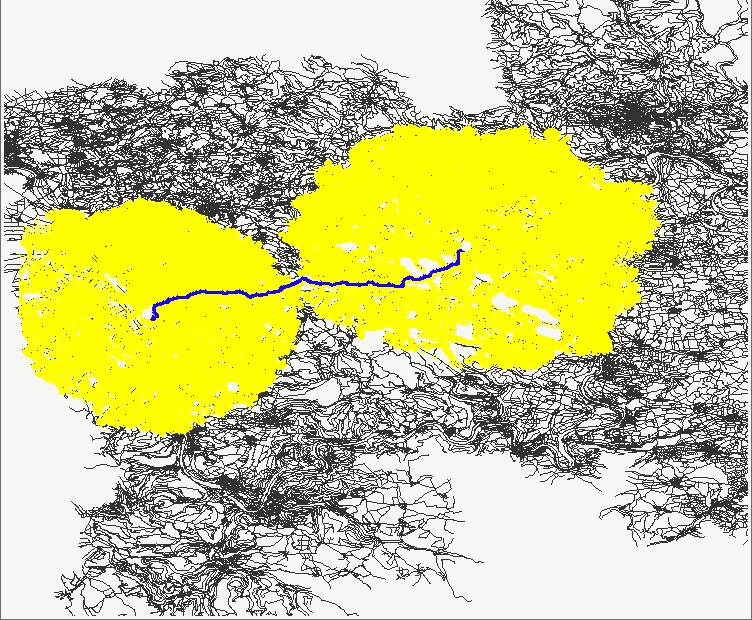
\includegraphics[height=15em]{bidijkstra-city}
    \caption{Dijkstra's Algorithm}\label{fig:bidijkstra}
\end{subfigure}
\hspace{2em}
\begin{subfigure}[b]{0.4\textwidth}
    \centering
    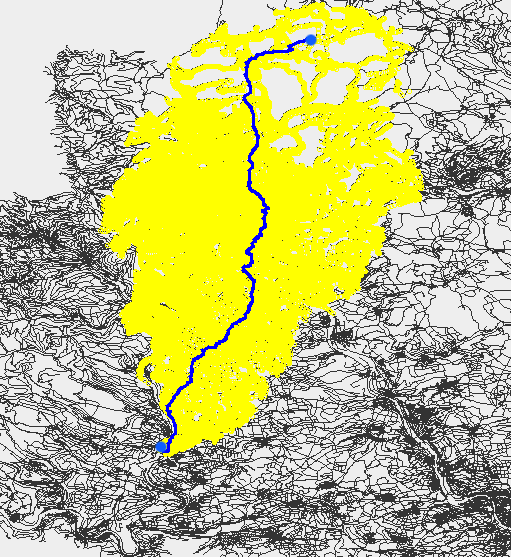
\includegraphics[height=15em]{astar-city}
    \caption{A* Algorithm}\label{fig:astar}
\end{subfigure}
\caption{Paths searched by each algorithm}
\end{figure}

\subsubsection{Contraction Heirarchies}

If the weights on each edge of the graph are known in advance, we can process
the graph to pre-compute the shortest path between certain key nodes in the
graph. One such algorithm for this is the Contraction Heirarchies algorithm,
which works by building shortcuts on top of each other in a heirarchy. It then
uses a modified version of bidirectional Dijkstra's algorithm that only uses
shortcuts higher than the current one to route between two points.

Although they double memory usage, in practice Contraction Heirarchies have a
huge impact on query times. For routing from Moscow to Madrid, any dijkstra
based algorithm takes at least 10 seconds, compared to less than 0.05s for a
processed graph.
\textbf{Cite: https://graphhopper.com/public/slides/2014-locationtech.pdf}

\subsection{Multi-Vehicle Routing Algorithms}

Providing viable routes for a single vehicle is now essentially a solved
problem, with various implementations used in many commercial products for both
consumers and businesses. However, the problem of routing multiple vehicles
simultaneously has many solutions~\cite{beejama,rt:compstudy,rt:decentralized,
rt:guidance,rt:congestion,rt:car,rt:unexpected}, but no accepted `best practice'
technique.

Multi-Vehicle routing algorithms come in various forms, depending on the
author's goals and expectations for future vehicle connectivity. Some algorithms
are designed to have a large scale overview of where each vehicle is on the
road, and will dispatch routing information to the vehicles centrally. On the
other end, algorithms may assume no central information and instead rely upon
vehicle to vehicle connections for passing information.

Multi-vehicle routing algorithms rely on some kind of network for optimised
routes to be created. These networks are referred to as \textbf{V2V} (Vehicle to
Vehicle) or \textbf{V2I} (Vehicle to Infrastructure) networks, and an algorithm
that relies on one or the other is known as a V2V or V2I algorithm.

\subsubsection{VANET}

A VANET (Vehicular-AdHoc NETwork) is a high-level use of V2V communication.
Although primarily theoretical at the moment, wireless networking protocols and
algorithms have been designed to support the creation and ues of a VANET. VANETs
have a number of potential use cases - allowing vehicles to follow one another
with no driver intervention, realtime calculation and distribution of traffic
information and so on.

Algorithms for multi-vehicle routing making use of VANETs have also been
created.

Modern simulation engines are often designed to support both V2V and V2I
algorithms - these engines are known as V2X engines.

\subsubsection{BeeJamA}\label{sec:beejama}

The BeeJamA~\cite{beejama} algorithm is a V2I approach for multi-vehicle routing. It is based
off an algorithm originally created for routing in packet switching networks
that has been adapted for use on road networks. Its behaviour is inspired by the
behaviour of bees, which are able to effectively search and scavange for food in
a large area surrounding their hive.

\noindent
\begin{wrapfigure}{l}{0.5\textwidth}
    \begin{greybox}
        \centering
        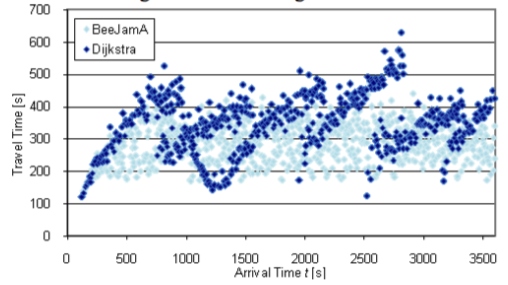
\includegraphics[width=\textwidth]{beejama}
        \caption{A comparison of BeeJamA to Dijkstra's Algorithm in terms of travel time.}\label{fig:bjam-dijkstra}
    \end{greybox}
    \vspace{-2em}
\end{wrapfigure}

The BeeJamA algorithm uses a quality rating function to determine a probablity
that a vehicle will be sent down a specific road. The map is split into regions
called Foraging Regions. Each region stores two types of table - an
Intra-Foraging Region routing table and an Inter-Foraging Region routing table.
These store the cost from the quality rating function of using a particular
route to reach the destination. The tables are kept up to date by sending
virtual vehicles between regions, which record how long their journey took and
inform the region they have entered.

Whilst routing, each vehicle consults the routing table and probablistically
picks its next step. This is a key part of the algorithm that helps keep routes
uncongested - if every vehicle took the optimal path, it would no longer be
optimal as it would have high levels of congestion. Results from a custom-built
simulation engine have shown that the algorithm can perform better than using
Dijkstra's algorithm with delayed traffic information.

\subsection{Nagel-Schreckenberg Model} \label{sec:nagel}

The Nagel-Schreckenberg Model~\cite{nagel} is a cellular automaton model for the
flow of traffic on roads.

The model splits roads into discrete cells, with each car taking up a single
cell at a time. The vehicles then follow 4 rules, in parallel to simulate the
flow of traffic. Each car has a fixed velocity $v$ for that step, which
represents the number of cells the vehicle will move forward in the final rule.
The model does not allow for overtaking, and as a result exhibits realistic
behaviour for traffic jams and flow.

\begin{enumerate}
    \item \textbf{Acceleration} - if the vehicle is not at the max speed and
        there is enough space ahead, increase the velocity by 1.
    \item \textbf{Slowing down} - if there is a vehicle nearer than the current
        velocity, reduce velocity to one cell less than the distance to the
        vehicle in front.
    \item \textbf{Randomization} - reduce the velocity by 1 with probability
        $p$.
    \item \textbf{Car movement} - move each vehicle forward by its velocity $v$.
\end{enumerate}

Each cell is meant to approximately represent the size of a single vehicle,
whilst each step (running through all four rules) represents a discrete amount
of time.

We'll now run through a brief example of the effects of each step. Our road will
have 9 cells with two vehicles on them. Our max speed ($v_{max}$) will be 5.
For this example, we will ignore the randomization step.

\begin{figure}[!h]
\centering
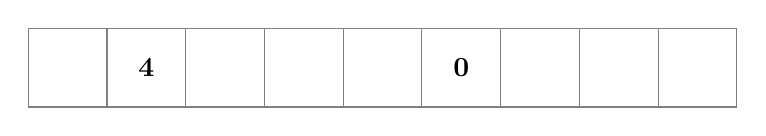
\begin{tikzpicture}
    \draw[step=1cm,color=gray] (0,0) grid (9,1);
    \node at (1.5,0.5) {\textbf{4}};
    \node at (5.5,0.5) {\textbf{0}};
\end{tikzpicture}
\end{figure}

We now perform the acceleration step for each vehicle. The second cell vehicle
is currently at speed 4 - as the vehicle in front is only 3 cells away, it does
not accelerate. The sixth cell vehicle increments its speed from 0 to 1.

During the slow step, the second cell vehicle must reduce its speed from 4 to 3
so it does not hit the sixth cell vehicle.

\begin{figure}[!h]
\centering
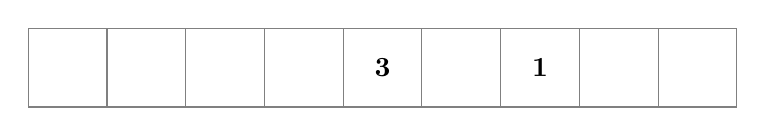
\begin{tikzpicture}
    \draw[step=1cm,color=gray] (0,0) grid (9,1);
    \node at (4.5,0.5) {\textbf{3}};
    \node at (6.5,0.5) {\textbf{1}};
\end{tikzpicture}
\end{figure}

Finally, the vehicles move to their new destinations. This demonstration breifly
shows the behaviour of two vehicles, but fails to demonstrate the creation and
flow of traffic jams. In Figure \ref{nagel-demo}, we can see how traffic jams
form and move in the Nagel-Schreckenberg model. This graph shows what happens
when there is a density of 0.1 cars per cell.

\begin{figure}[h]
    \centering
    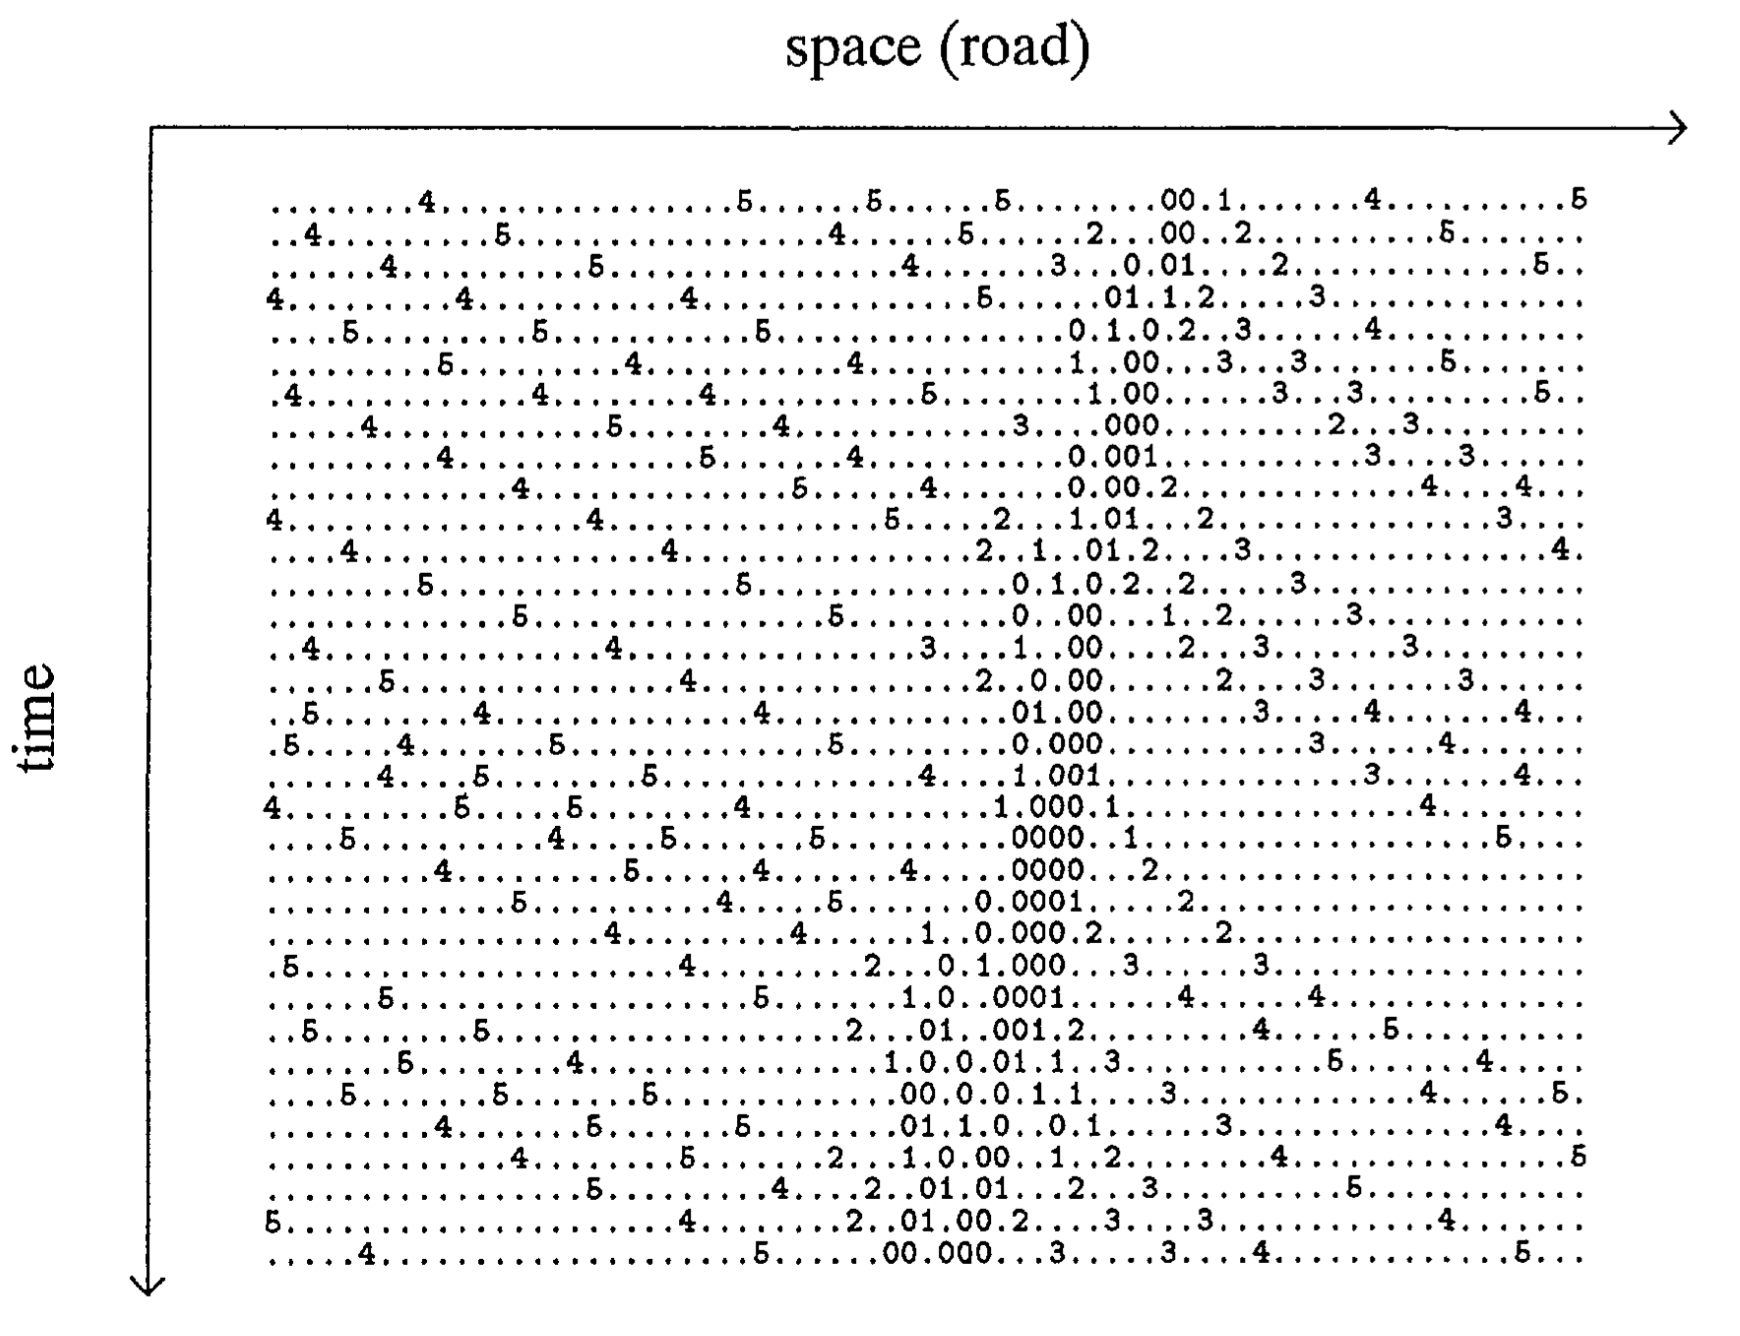
\includegraphics[scale=0.4]{nagel}
    \caption{Formation of traffic jams in the Nagel-Schreckenberg Model}\label{nagel-demo}
\end{figure}

\section{Implementation Background}

\subsection{OpenStreetMaps}

In OpenStreetMaps, there are three main elements - nodes, ways, and relations.
Each of these can have certain tags that describe the real-world object they
represent. For example, a way could have tags describing it as a highway with 3
lanes, whilst a node could have tags identifying it as a park bench or phone
booth.

A standalone node is usually a single entity with a latitude and longitude as
well as an ID. By themselves, they can be used to represent small features such
as traffic lights, lampposts, or pylons. However, a way is also defined by an
ordered list of nodes.

Ways are the most flexible element in OpenStreetMaps. If a way starts and ends
at two different nodes, it is called an `open' way. This is commonly used for
sections of roads and paths. A way that starts and ends at the same node is
called a `closed' way. Often this is used to represent an area - such as a park
or the shape of a building - but can also be used for roundabouts and circular
barriers. There are tags for identifying if a closed way is an area or not
(primarly the \texttt{area=yes} tag, but many things are defined as areas even
without this tag).

Finally we have relations. These are the most complex type of element, holding
an ordered list of ways, nodes and other relations and have tags for describing
the relationship between them - for example, a bus route could be described as a
list of ways and nodes. For the purposes of routing, it is only important to
know that relations are used for turn restrictions - the rules that define which
directions a vehicle may move from one road onto another. This is important for
routing much more than mapping, as users would be frustrated to find that a
route they had expected to travel on is illegal or unsafe in practice.

\subsection{GraphHopper Routing Engine}

GraphHopper has been built to be fast, flexible and powerful. It covers the full
flow of creating a custom routing service - from parsing and importing
OpenStreetMaps data, processing the network for performance improvements,
routing using multiple dijkstra and A* algorithms and running a web server for
making requests. Additionally, it has built in support for car, bicycle,
pedestrian and other types of travel as well as the ability to create custom
vehicle types.

\begin{figure}[p]
    \centering
    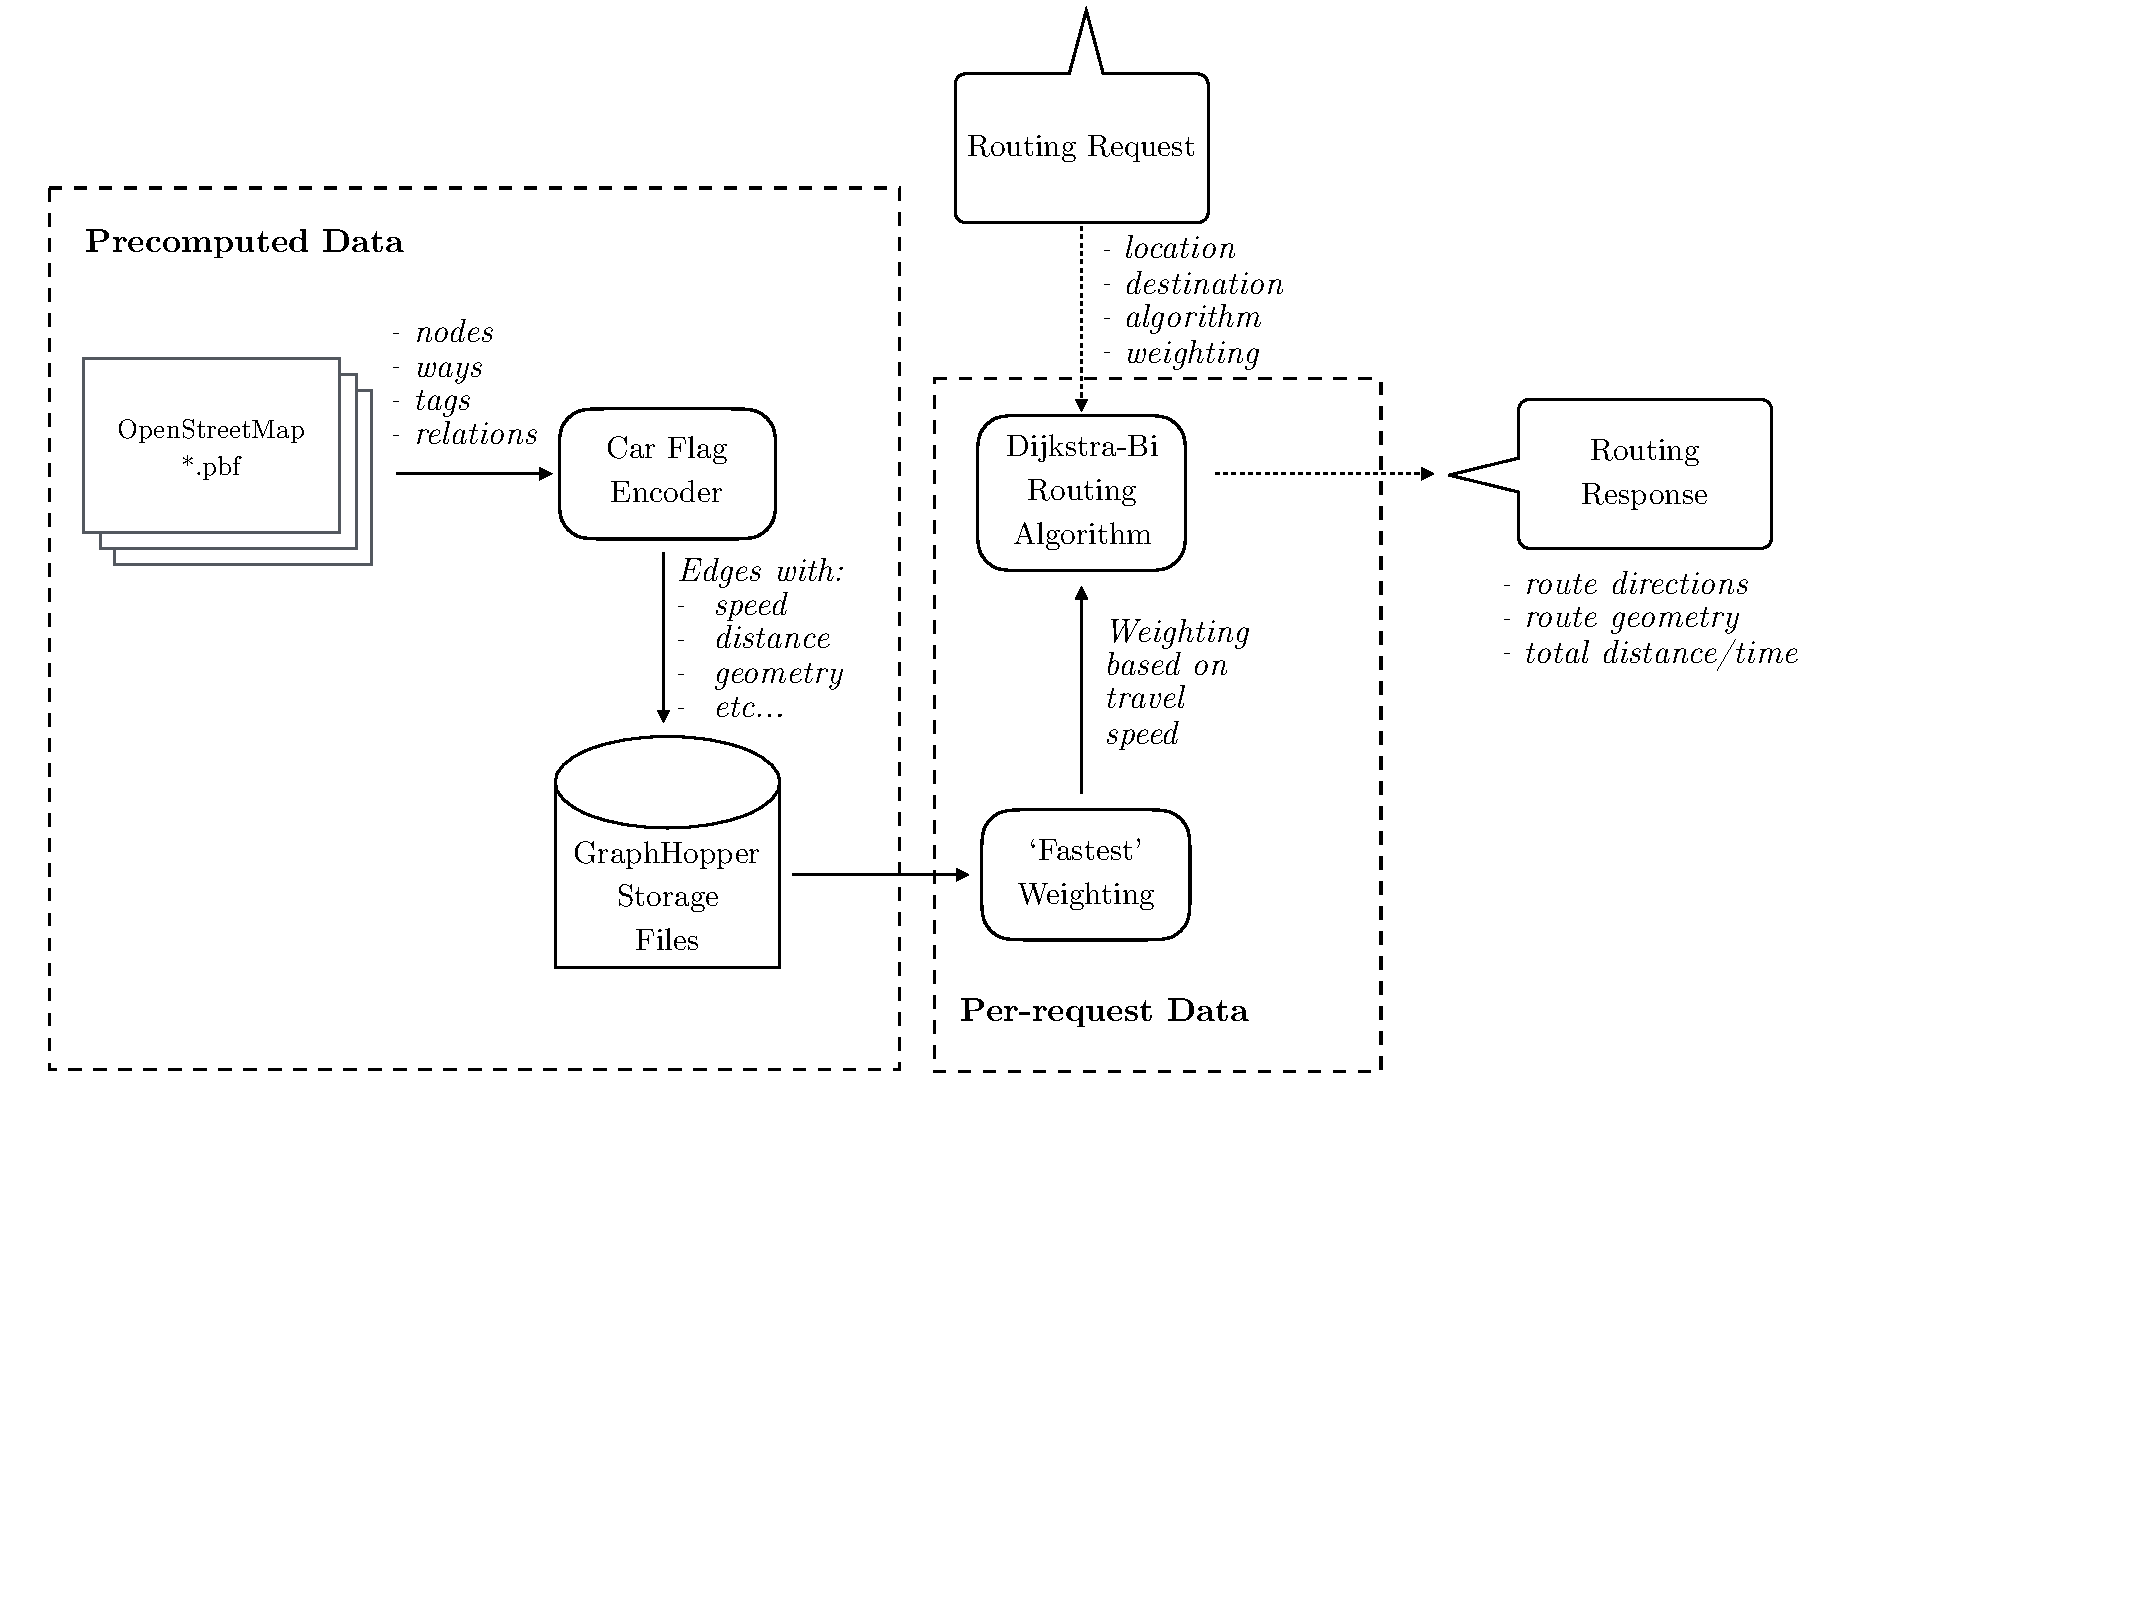
\includegraphics[scale=0.5,page=1,clip,trim=0 8cm 4cm 0]{architecture}
    \caption{An overview of the GraphHopper Architecture}\label{fig:gh-arch}
\end{figure}

Figure \ref{fig:gh-arch} shows the salient parts of the architecture for this
project.  Note that we are not using the web or android modules, so no details
regarding their functionality has been included. For the most part, the use of
routing will be relatively high level - simply requesting a list of edges
between two points. However, the underlying engine also has a number of features
that make it easy to customise, which will be used for more complex situations.

It is important to note that the conversion from OSM data to GraphHopper data is
done only once (as it is a time consuming process) and stores its results on
disk.

\subsubsection{OpenStreetMap Encoding}

\begin{figure}[p]
    \centering
    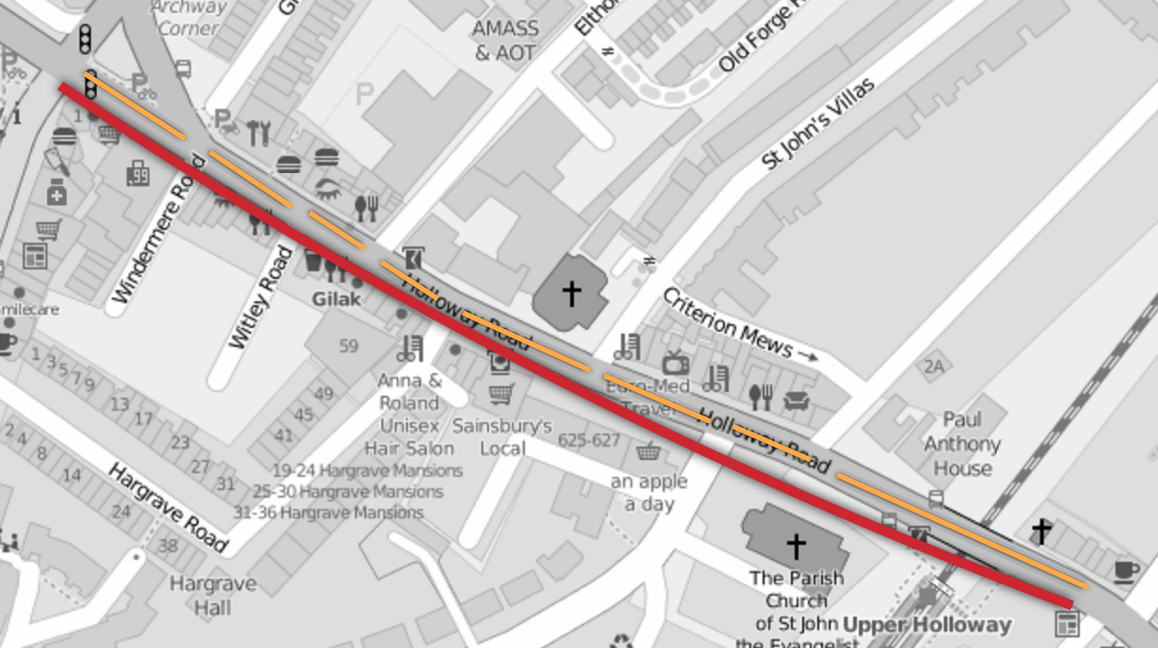
\includegraphics[scale=0.6]{osm-gh}
    \caption{OpenStreetMap way representation compared to edges in GraphHopper}\label{fig:osm-gh}
\end{figure}

The first thing to understand is how GraphHopper converts the OpenStreetMap data
into a graph that can be used for routing.  For the purposes of routing, we are
primarily concerned with ways that represent roads. However, a way does not
represent the entirety of a given road - but is also not granular enough to
allow routing. Figure \ref{fig:osm-gh} shows the difference between ways, roads
and edges. We can see that the physical Holloway Road extends beyond the OSM way
(red). However, if we used the way for routing we could not route from Hargrave
Road to St John's Villas via Holloway Road. To perform routing, GraphHopper
splits every way into an edge whenever there is a junction. GraphHopper's edges
can be seen in orange. These can be used to perform the routing calculation
mentioned above - there is now an edge along a subsection of Holloway Road that
conncets Hargrave Road to St John's Villas.

\subsubsection{Flag Encoders}

Internally, GraphHopper compresses the information about each edge into a single
integer - so each edge takes up no more than 32 or 64 bits.

The \texttt{FlagEncoder} interface (and the \texttt{AbstractFlagEncoder} class)
define what operations have to be done to convert a section of a way into an
edge. Edges store a few key pieces of information - by default, GraphHopper
stores the length, speed and ID of an edge, with additional information
optionally stored by the flag encoder itself.

For example, the \texttt{CarFlagEncoder} uses the type of road to calculate the
correct maximum speed of the vehicle and then sets the speed for the edge, using
5 bits. The \texttt{MotorcycleFlagEncoder} can do the same thing, but with
different speed values for each type of road. The concept can be extended to
storing even more information at each edge - for example, 3D graph data can be
stored for bike and walking routes, whilst a FlagEncoder for trucks could store
height, weight, width and length restrictions to ensure safe travel.

\subsubsection{Weightings}

Flag Encoders are used to define what information can be used whilst routing -
but this data is fixed once the OSM file has been processed. A weighting defines
how the data stored at the edges is used. For example, one can search for the
shortest route, the fastest route, or a custom weighting that incorporates other
information stored in the edge.

\subsubsection{Routing Requests}

As it is primarily designed to work with its web module, GraphHopper uses a
request-response pattern for requesting and receiving routes.

\begin{lstlisting}[label=lst:gh-route,caption={GraphHopper request and response}]

GHRequest ghRequest = new GHRequest(startLat, startLon, endLat, endLon);
ghRequest.setWeighting("fastest");
ghRequest.setAlgorithm("dijkstrabi");
GHResponse ghResponse = graphHopper.route(ghRequest);

\end{lstlisting}

The \texttt{GHRequest} class stores all the information required to make a
routing request, including the weighting and algorithm to use. An example of its
use can be seen in Listing \ref{lst:gh-route}.

The response is returned in a \texttt{GHResponse} class, which holds information
about the route in a number of different ways. The user is also responsible for
checking the \texttt{hasErrors} method before requesting the route itself.  Once
this has been done, the route itself can be read.

As GraphHopper supports the use of an alternative routes algorithm (meaning a
single request can respond with more than one route), the GHResponse class has
both a \texttt{getAll} and \texttt{getBest} method, which return a list of
\texttt{PathWrapper}s and a single PathWrapper respectively. The PathWrapper
holds the route itself as well as some metadata. The route can be accessed as a
list of instructions or as the raw list of points for visual display.
Additionally, the total distance and time of the route are recorded.

However, GraphHopper does not provide a list of edges or of OSM Ways that are
included in the route. Internally, the list of edges is calculated with the
\texttt{calcPaths} function, which returns a list of \texttt{EdgeIteratorState}
objects. These objects are fundamental to the way the graph is stored an
accessed in GraphHopper.

GraphHopper uses the flywheel pattern for efficient access to graph data. The
EdgeIterator and EdgeIteratorState class are the primary way of interacting
directly with the edge data. EdgeIteratorState is an interface containing
getters and setters for the edge ID, its geometry, the flags stored by the
FlagEncoder, and the name of the road the edge is a part of. It also allows
access to the nodes at either end of this edge. The node at the start of the
edge is called the Base Node, whilst the node at the end of the edge is the
Adjacent Node.

% -----------------------------------------------------------------------------

\chapter{Project Execution}
\label{chap:execution}

%%%%%% ======= 15 PAGES ======= %%%%%%

\section{Overview}

The execution of this project was split into 4 stages, each with its own goal.

\begin{enumerate}
    \item \textbf{Initial Implementation} - create the inital client and
        server with vehicles moving on a map.
    \item \textbf{Realistic Simulation} - implement the Nagel-Schreckenberg
        model to make the vehicle behaviour more realistic.
    \item \textbf{Performance and Architecture Improvement} - make the
        simulation engine fast and flexible enough to deal with the challenges
        of algorithm design.
    \item \textbf{Algorithm Design and Implementation} - creating and improving
        a novel approach to the multi-vehicle routing problem using the
        simulation engine.
\end{enumerate}

\section{Initial Implementation}

The initial implementation had a few key goals, with the primary objective of
having basic vehicles moving on a map. This stage was essentially a way of
setting up the basic archictecture of the project, without finalising the
details of how routing algorithms would be implemented.

\subsection{Architecture Design}

\begin{figure}[h]
    \centering
    \includegraphics[scale=0.5,page=2,clip,trim=0 17cm 3cm 0]{architecture}
    \caption{The initial architecture for the simulation engine}\label{fig:init-arch}
\end{figure}

Figure \ref{fig:init-arch} shows a simple architecture diagram for the initial
implementation of the engine. Once the client has made a request to the engine,
it sets up and starts routing the vehicles. Each vehicle is responsible for
storing and updating its own position on each timestep. This data is converted
into a string and sent to the client, which then moves each vehicle on the map.

One of the goals of this project was to make it possible to visualise and
simulate at the same time. This naturally lends itself to a client-server
architecture, and with the rate of improvement of modern web browsers it seemed
like a wise choice to use a browser for the visualisation component.

This also means that the server can be run remotely with no additional setup -
more computationally expensive algorithms could be run on high-powered servers
with the results still visible locally for the user.

\subsection{Project Setup and Modularisation}

When setting up the project, it was important to be able to use and modify the
underlying GraphHopper routing engine. The GraphHopper project is setup with
four existing modules - core, tools, web and android. Although it would have
been ideal to use GraphHopper as an external library, it was necessary to make
minor internal changes to the main engine. As such, I created a GitHub fork of
the project and added marmoset as a fifth module in the project.

GraphHopper uses the Maven dependency and build tool, with its own custom shell
script for building, running and testing different versions of the engine. To
keep Marmoset separated from the core project, I created my own shell script for
building and running the marmoset engine. It supports four main actions - clean,
build, rebuild and run. It also allows multiple commands to be run in succession
for convenience.

Additionally, I wanted to create a modern codebase in spite of the core engine
being written in Java. Although I briefly explored using Scala, much of my work
would rely on extending and using the existing Java APIs in GraphHopper.
Thankfully, Java 8 has introduced a number of key tools that allow
functional-style code to be written. The code below shows the difference for
performing a simple task - converting a list of objects into strings and joining
them by commas.

\noindent
\begin{tabular}{c|c}

\begin{lstlisting}
public String getVehicleData()
{
    StringBuilder sb = new StringBuilder();
    for (VehicleController v : vehicles)
    {
        sb.append(v.getVehicle().toString());
        sb.append(",");
    }
    // remove last comma
    sb.deleteCharAt(sb.length() - 1);
    return sb.toString();
}
\end{lstlisting} &
\begin{lstlisting}[boxpos=b]
public String getVehicleString()
{
    return vehicles.stream()
        .map(Vehicle::toString)
        .collect(Collectors.joining(","));
}
\end{lstlisting} \\ \vspace{1em}
Java 7 Implementation & Java 8 Implementation \\
\end{tabular}

Here we can see how six lines of code can be condensed into a single, more
readable line using the Java 8 Stream API.

\subsection{Server Implementation}

For the raw file server, I used the NanoHttd~\cite{nanohttpd} library, as it
requires minimal setup and is easy to run on a separate thread. For the
client-server communication, I initially used the NanoHttpd WebSocket
implementation, but it did not appear to be fully functional. As such, I
switched to using the Java-Websocket library~\cite{javawebsocket}, extending the
WebSocketServer class to create the MarmosetSocketServer class.

In the architecture diagram (Figure \ref{fig:init-arch}), we see four main
classes on the backend.

The \texttt{MarmosetSocketServer} class handles the connection between server
and client.  It keeps track of each of the connected clients and offers a simple
command to distribute vehicle position data to each of them.

The \texttt{Marmoset} class is a static class that is the main entry point for
the program. It initialises the file server and WebSocket server, and creates a
new thread for running the MarmosetHopper timesteps. It also handles passing
data from MarmosetHopper to the socket server.

In most types of simulation, time must be split into discrete steps that
represent a fixed time interval in the real world. Looking at Figure
\ref{fig:init-arch}, we can see that it is the Marmoset class that triggers each
timestep. At this stage of the project, I had not established how well the front
or back end would perform. As a way of simplifying the data flow and processing,
Marmoset simply waits one second between each call of the timestep function.  As
both front end and back end take significantly less time than a second to
perform their tasks, this was an appropriate simplification for this stage of
development.

The \texttt{MarmosetHopper} class holds the list of vehicles and and creates an
instance of the GraphHopper routing engine. It initialises all the vehicles,
instructs them to update on each timestep and gathers their position information
together to be sent to the clients.

When initialising the vehicles, the starting location and destination are chosen
as random latitude and longitude co-ordinates within London.

Finally, the \texttt{Vehicle} class represents a single physical vehicle on the
map. Each vehicle holds its location and the route it plans to take. The routing
information is obtained by requesting a route from GraphHopper. The route is
returned in a number of ways, including as a list of points that can be used to
draw the route. This does not include the speed of each road travelled, so
cannot be used for realistic simulation. However, for this initial
implementation the location is updated on each timestep by simply moving to the
next point in the list. This is very innacurate, but it does allow us to verify
the functionality of all parts of the system without touching the details of
routing. The vehicles return their location as a string containing their id,
latitude and longitude.

\subsection{Client Implementation}

When loading the web page, a map is created and centered on the correct
location.  The client then connects to the WebSocket back end and listens for
data. When it receives the vehicle data, it creates or updates the position of
each vehicle marker.

The Leaflet.js~\cite{leaflet} library is used for both map and marker creation.
A simple \texttt{Car} class has been created to keep track of the location of
each marker. It stores a reference to the Leaflet.js Marker object and provides
a method to move the marker to a new location. The
Leaflet.AnimatedMarker~\cite{animarker} library handles smoothly moving the
points to their next location, making the cars look like they're driving around
the map in real time.

Meanwhile, A single \texttt{CarSet} object connects to the WebSocket server and
stores the Car objects. When data is recieved, it creates new Cars or updates
the position of existing vehicles using their \texttt{moveTo} method.

\subsection{Results and Improvements}

\begin{figure}[h]
\centering
\begin{subfigure}[b]{0.4\textwidth}
    \centering
    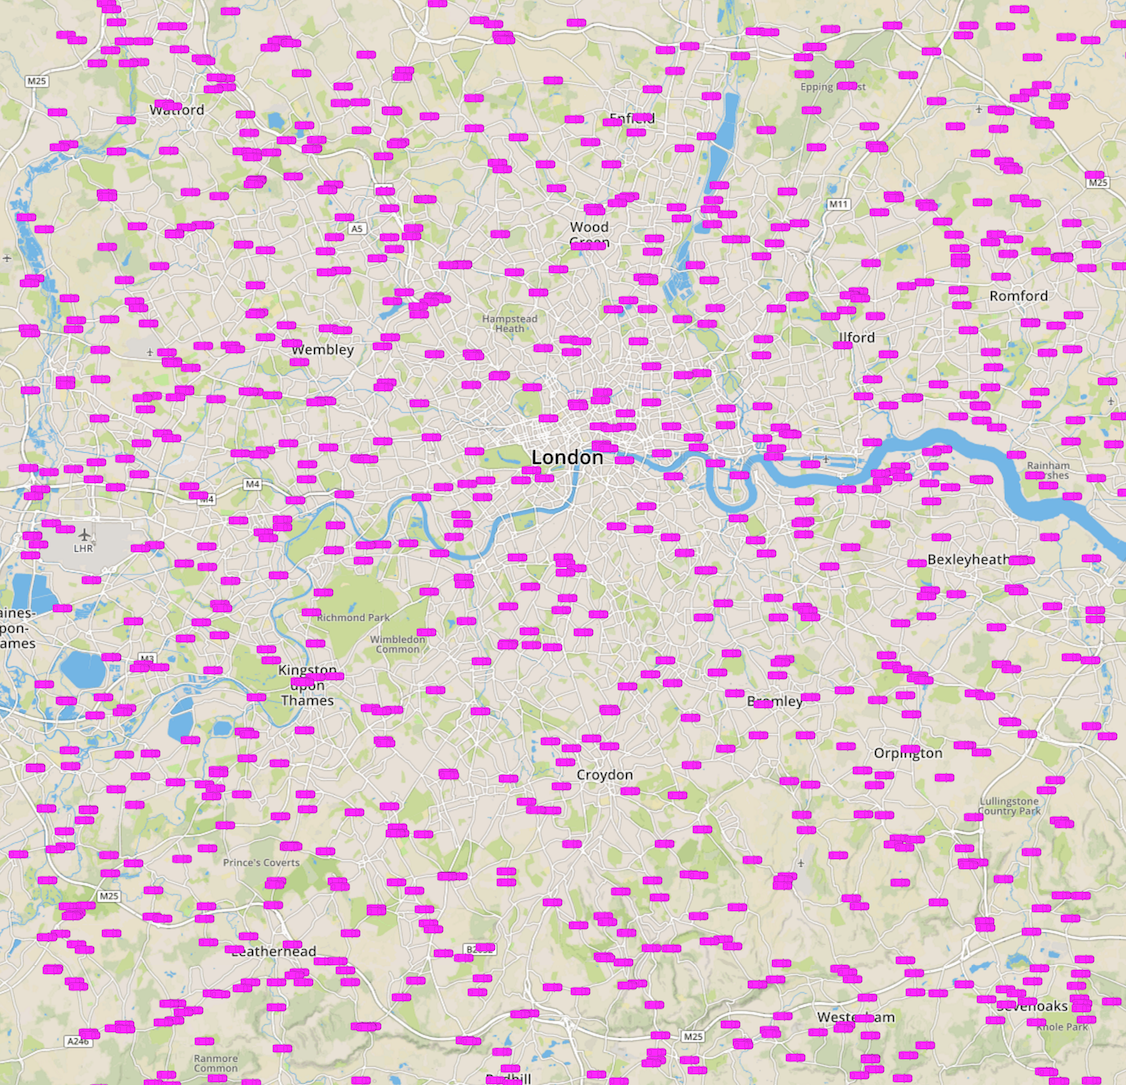
\includegraphics[height=15em]{init-start}
    \caption{10th Iteration}\label{fig:init-start}
\end{subfigure}
\hspace{2em}
\begin{subfigure}[b]{0.4\textwidth}
    \centering
    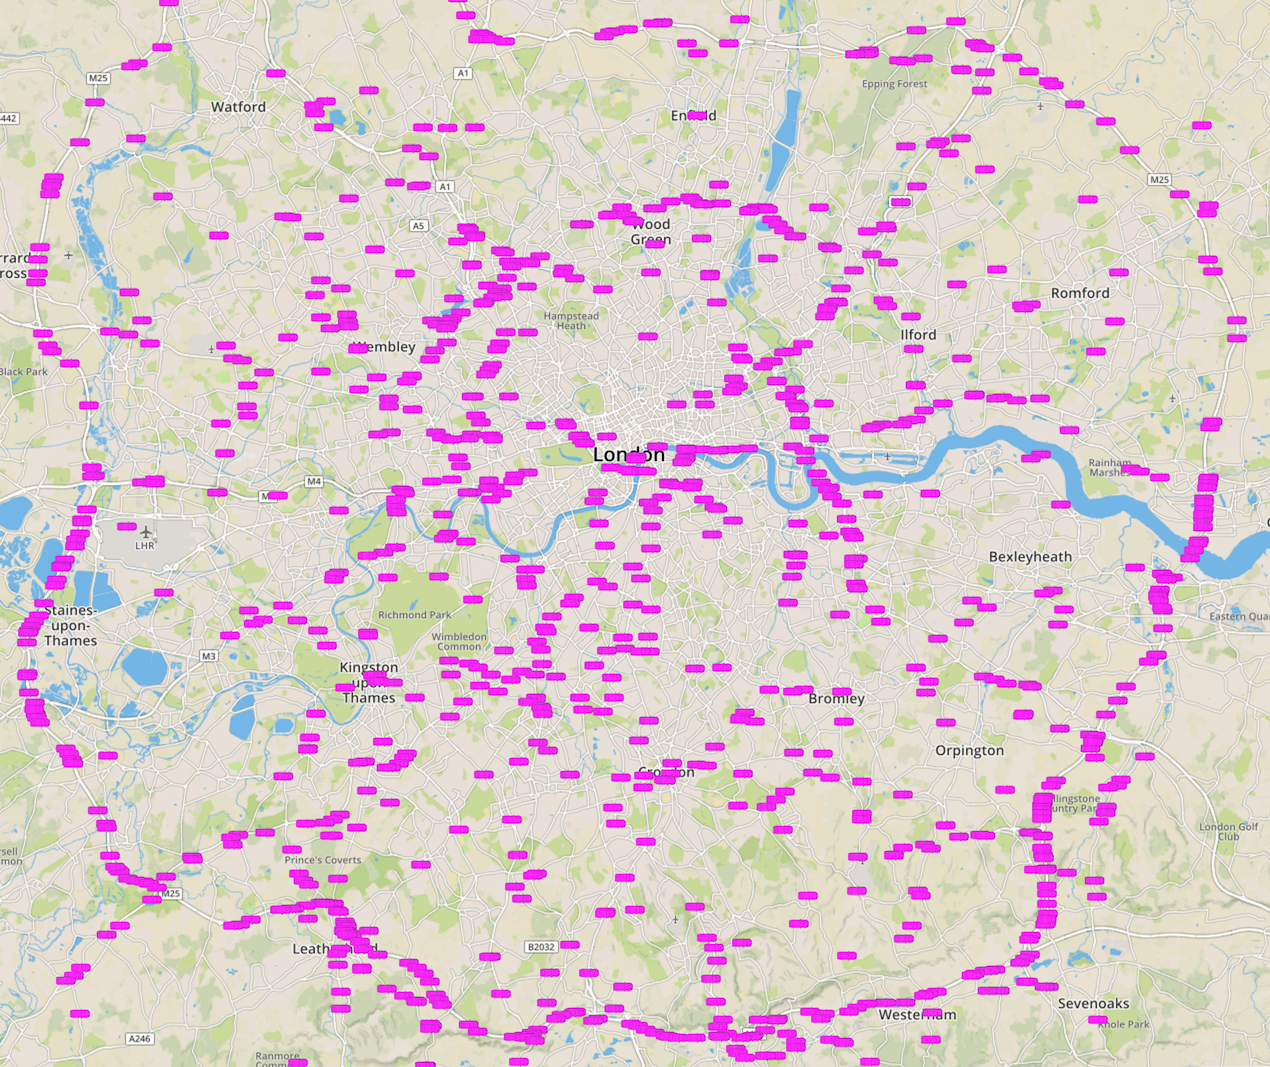
\includegraphics[height=15em]{init-200}
    \caption{200th Iteration}\label{fig:init-200}
\end{subfigure}
\caption{Vehicle positions at different iterations}
\end{figure}

At the end of this section of the project, the engine was capable of performing
its core task of simulating and visualising vehicles. In spite of many of the
simplifications in the system, it provides quite realistic results -
\ref{fig:init-200} shows that even after a small number of iterations certain
roads become more congested than others. This matches the reality of driving on
London roads - the M25 and North Circular suffer frequent delays due to a high
volume of vehicles driving on them.

However, there are many core features missing from the engine at this point.

\begin{itemize}
    \item The engine simulates a fixed number of vehicles (1000) - no more can
        be added or removed.
    \item Vehicles do not move realistically. As they simply jump to the next
        point on their route, a curved path would take much longer to travel
        than a straight one.
    \item Vehicles are independent. Vehicles travel on their own with no sense
        of traffic or congestion.
    \item The timestep is fixed to one second, even though the actual processing
        takes substantially less time for both front and back end.
    \item Metrics are not tracked. Other than watching the simulation, there is
        no further understanding that can be gained from simulating.
    \item The simulation cannot be paused without terminating it and starting
        again.
\end{itemize}

For the next stage of development, I focussed on improving the realism of the
vehicle simulation.

\section{Realistic Simulation}

In section \ref{sec:nagel} we introduced the Nagel-Schreckenberg Model for
traffic flow simulation. This section discusses the implementation of this model
on top of the existing simulation engine described above.

The original model is designed for a single road, either in a loop or an
extended straight stretch. Implementing this on a road network introduces some
additional challenges, particularly when dealing with the integration with
GraphHopper and OpenStreetMaps.

The two main concerns are how the cells should be stored and how the cells
should be used in conjunction with the routes created by GraphHopper.

\subsection{Cell Storage}

A number of techniques for storing the cells were considered. Firstly, we must
consider how we create edges. We have the option of using either GraphHopper
edges - which are small, but do not have junctions - or OSM ways, which can be
larger but would allow for more usable metrics and would make the system less
dependent on GraphHopper.

Ultimately, I chose to use GraphHopper's edges as the base unit for cells. This
is primarily due to the fact that GraphHopper does not have an internal mapping
from its edges to OSM Ways, and does not return which Ways are used as part of a
routing response. Additionally, GraphHopper provides an
\texttt{AllEdgesIterator} that returns both the maximum edge ID as well as the
data for every edge in the graph.

The next decision is how and where to store the cells. In the original paper, we
saw that each vehicle was represented by its velocity stored as an integer in
the cell array. As we are storing a much larger amount of information about each
vehicle in the Vehicle class, this is not a viable option. If vehicles store
their own velocity and keep track of the current edge and cell they are on, the
cells only need to know if any vehicle is present in a cell. As such, each cell
is simply a boolean value in an array. The cell is set to \texttt{true} if a
vehicle is in the cell and \texttt{false} if the cell is empty.

In terms of physical storage, the are a number of options. At its core, we need
a mapping from edge IDs to cell arrays. In Java, this would usually be
represented as a Map of Lists (\texttt{Map<Integer, List<Boolean>>}). However,
the edge IDs in GraphHopper have been designed to be sequential starting from 0,
with the highest ID accessible from the AllEdgesIterator. This means that we can
instead use a list of lists (\texttt{List<List<Boolean>>}). This has the
advantage of allowing the lists to grow in size dynamically, but may have
performance issues. In Java, Lists must store other Object types rather than
primative types. As objects in Java are all pointers, each Boolean will require
a pointer to a separate memory location that holds the true or false values.
This is likely to harm cache performance, something particularly important given
the frequency that the cells will be accessed.

Instead, we can simply allocate a two-dimensional array of booleans for each
edge as a raw array. This avoids the issues with pointers and is consistent with
the way GraphHopper stores edges.

\begin{wrapfigure}{r}{0.45\textwidth}
    \begin{greybox}
    \begin{center}
        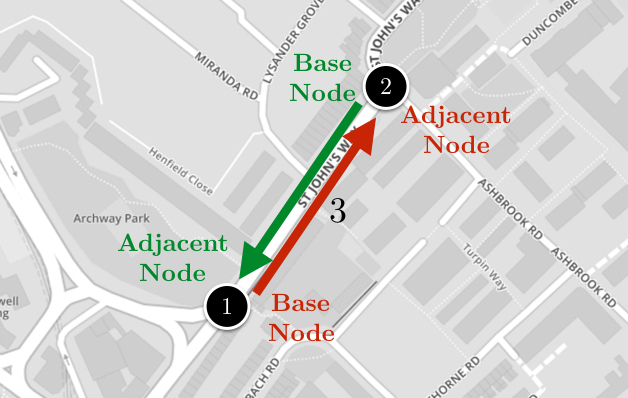
\includegraphics[width=\textwidth]{gh-edge-problem}
    \end{center}
    \caption{The problem with GraphHopper edges}\label{fig:gh-edge-problem}

    \vspace{0.6em}
    In the diagram above, we see two nodes (with ID 1 and 2) joined by an edge
    (with ID 3). Imagine we've performed two routing requests, one in red and
    one in green. Both routes go through edge 3, but in opposite directions.
    However, both edges will return true from the \texttt{isForward} method of
    EdgeIteratorState, despite going in opposite directions. Although
    GraphHopper knows that one of these is in reverse, the data is hidden from
    us.
    \end{greybox}
    \vspace{-2em}
\end{wrapfigure}

However, there is another challenge with regards to storing the data. When
parsing the ways, GraphHopper identifies the direction of the edge - each edge
can support moving either forward or reversed. When a route is provided by the
routing engine, it is in the form of a list of EdgeIteratorStates. The
EdgeIteratorState class has been designed to hide the `true' direction of the
edge, instead switching which node is the base node and which is the adjacent
depending on the direction the vehicle is travelling in. The end result of this
is that every edge appears to be a forward edge when received from the engine.
For the cell model, we need to have two separate directions for the roads, or
vehicles going in opposite directions will crash into each other and block the
roads.

In Figure \ref{fig:gh-edge-problem}, we can see why this may be an issue. When
moving through the edges, we are unable to tell if we are travelling forwards or
backwards based on the EdgeIteratorState by itself - the ID is the same and the
\texttt{isForward} method returns true in both directions. Initially, I had
thought a more complex solution than the boolean arrays would be required -
perhapes some kind of 2D mapping from pairs of node IDs (or a base node and edge
node) to the cell array. However, it is important to note that we don't actually
need to know if GraphHopper internally stores an edge as forward or reverse so
long as we are able to distinguish between the two cases shown above.

The technique I came up with to solve this uses the fact that the base node and
adjacent node returned by the edge changes depending on direction. As such, we
can define edges where the base node is greater than the adjacent node as
`forward' and edges where the base node is less than the adjacent node as
`backwards'. This allows us to reliably differentiate between the forward and
backwards cases, and save the vehicles from crashing into each other.

The \texttt{CellGraph} class handles the storage for the cells, providing
convenient getters and setters for edges at specific cells. It also
transparently handles the forward and reverse edges, storing two boolean arrays
(\texttt{boolean[][] cells} and \texttt{boolean[][] reverseCells}) and uses
whichever one is appropriate for the current EdgeIteratorState.

\subsection{Vehicle and Cell Iterators}

\begin{figure}[h]
    \centering
    \includegraphics[scale=0.5,page=5,clip,trim=0 15cm 15cm 0]{architecture}
    \caption{The Nagel-Schreckenberg Model across edge boundaries.}\label{fig:nagel-multi}
\end{figure}

As we saw in Section \ref{sec:nagel}, one of the key parts of the
Nagel-Schreckenberg model requires vehicles to know how far they are from the
next vehicle. In \ref{fig:nagel-multi}, we see three vehicles - A, B and C.
Vehicle A is 2 cells from B and 3 cells from C. However, A is soon to turn left
onto the edge with C, meaning it should not consider B as ahead of it.

However, each of these paths consists of multiple edges. We need a way of
treating lists of edges as a single continuous array of cells. This is a good
use case for the iterator pattern, providing us with an abstraction over the
underlying arrays.

The \texttt{VehicleIterator} class is responsible for storing and moving through
the vehicle's route. It stores the list of EdgeIteratorState objects and moves
to the next element each time its \texttt{next} method is called. It implements
the EdgeIteratorState API for full compatibility with GraphHopper. In addition
to the usual EdgeIteratorState methods, it can return the road speed of an edge.

The \texttt{CellIterator} class stores the cell ID and the VehicleIterator,
meaning it can traverse across edge boundaries by calling the VehicleIterator's
\texttt{next} method. It also has a reference to the CellGraph so that it can
return weather there is a vehicle in the current cell.

%When routing, GraphHopper starts by finding the nearest edge to the start and
%end locations. It then creates `virtual edges' from the start location to the
%first edge and from the last edge to the

\subsection{Vehicle Class}

The Vehicle class now has five core methods that are used for running the
simulation, rather than the single \texttt{calculateStep} function used before.
The \texttt{accelerationStep}, \texttt{slowStep}, \texttt{randomStep} and
\texttt{moveStep} all correspond to the four steps of the Nagel-Schreckenberg
algorithm, whilst the \texttt{updateLocation} method interpolates the cell
location into the edge geometry to find the vehicle's location.

The vehicle class stores two core things that make the implementation possible.
The first is a VehicleIterator (named \texttt{route}) containing the list of
edges each vehicle will take, as well as its current edge. The second is the
current cell ID the vehicle is on. By duplicating the VehicleIterator and
passing it to a new CellIterator, the vehicle can find out if it is able to
accelerate or must slow down - even if the vehicle in front is multiple edges
ahead.

\begin{minipage}{\linewidth}
\begin{lstlisting}[caption={The \texttt{slowStep} implementation making use of the CellIterator},
                    label=lst:slowStep, numbers=left]
public void slowStep()
{
    int j = 0;
    CellIterator c = new CellIterator(new VehicleIterator(route), cg, cellId);

    while (!c.next() && j <= v)
        j++;

    if (j <= v)
        v = j;
}
\end{lstlisting}
\end{minipage}

Listing \ref{lst:slowStep} shows how the CellIterator and VehicleIterator work
in conjunction to implement the the slow step of the Nagel-Schreckenberg method.
The variable \texttt{j} represents the distance to the next vehicle, whilst
\texttt{v} is the vehicle's current velocity. Line 4 shows the initialisation of
the CellIterator - note that \texttt{route} is a VehicleIterator being created
with a copy constructor, meaning that the current location of the vehicle will
not be changed from this CellIterator.

\subsection{Results and Evaluation}

<CREATE ARCHITECTURE DIAGRAM YAH>

At this point, the system was capable of simulating any number of vehicles with
realistic traffic flow behaviour. However, there were still many key performance
improvements that needed to occurr before the system would be ready for
algorithm development.

\begin{itemize}
    \item The back end still waits one second per iteration.
    \item The back end archictecture does not allow for vehicles with different
        behaviour.
    \item The back end does not make optimal use of the multiple threads and
        cores that modern computers have available to them.
    \item The front end has graphical glitches and poor performance when
        showing more than 16,000 vehicles.
    \item Metrics for later data analysis are not recorded.
    \item Additional vehicles could not be added to the simulation once it had
        started.
    \item The simulation cannot be paused or resumed.
\end{itemize}

\section{Performance and Architecture Improvements}

There were two core goals for the system at this stage. Firstly, improve
performance such that at least 64,000 vehicles can be simulated and secondly,
modify the architecture of the system to support multiple vehicle types,
preferably with the ability to have different vehicle types running side by
side.

\subsection{Front-end Performance}

Before this stage of the project, the front end had many performance issues.
With enough vehicles, the entire page would become slow to respond and update.
Even with the one second delay, it would sometimes fail to update before
recieving the next set of data.

\begin{figure}[h]
\centering
\begin{subfigure}[b]{0.4\textwidth}
    \centering
    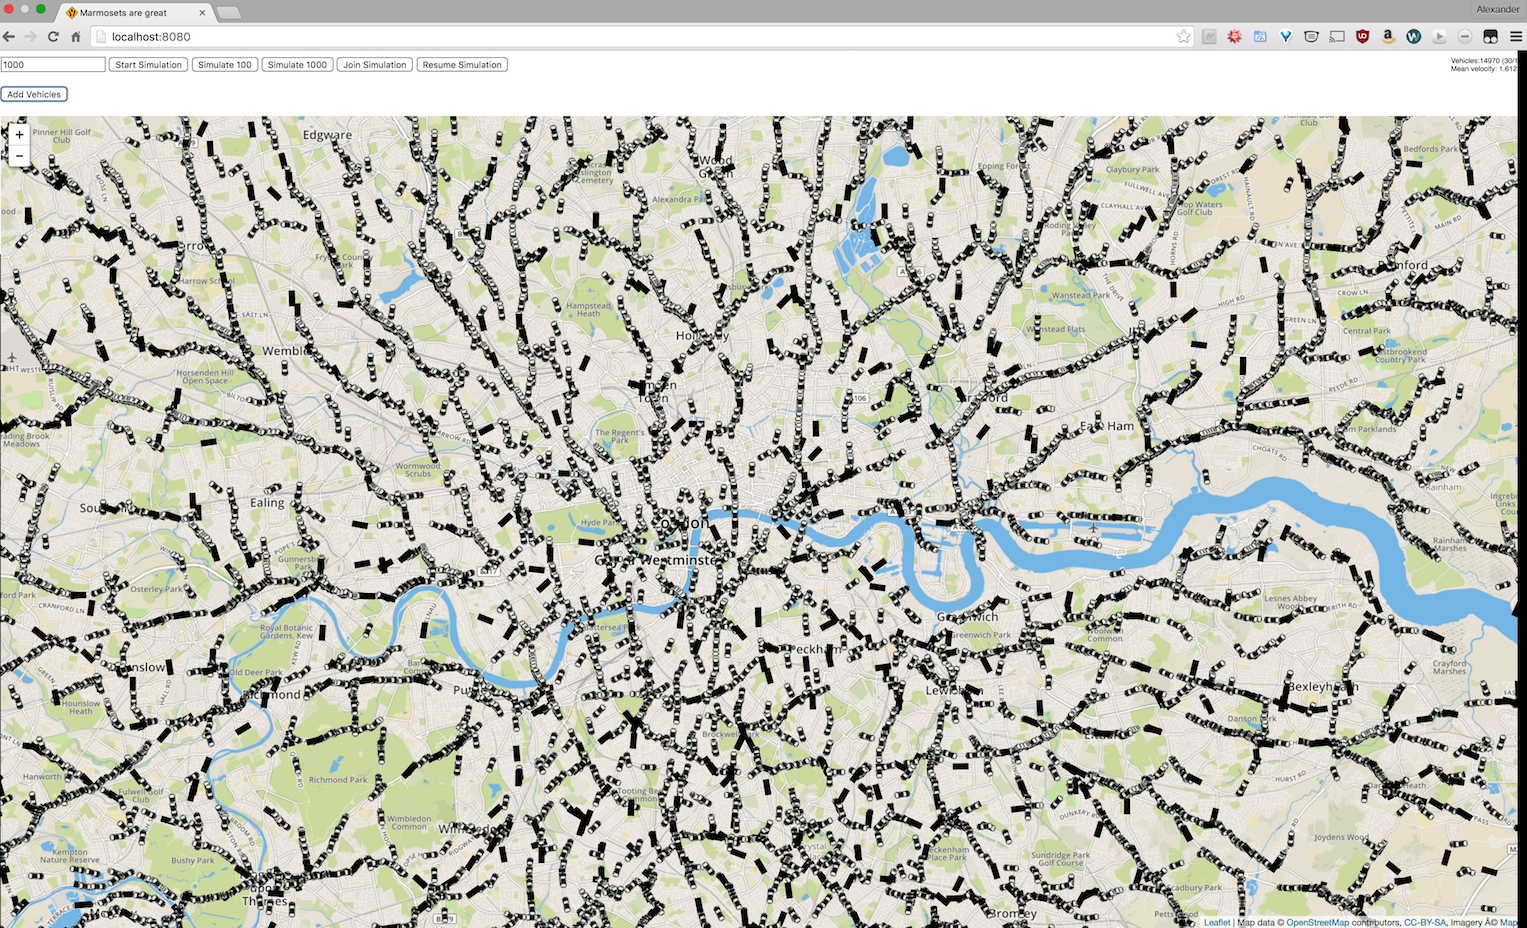
\includegraphics[height=9em]{glitches-car}
    \caption{Vehicles showing up as black squares rather than image icons.}\label{fig:glitches-car}
\end{subfigure}
\hspace{3em}
\begin{subfigure}[b]{0.4\textwidth}
    \centering
    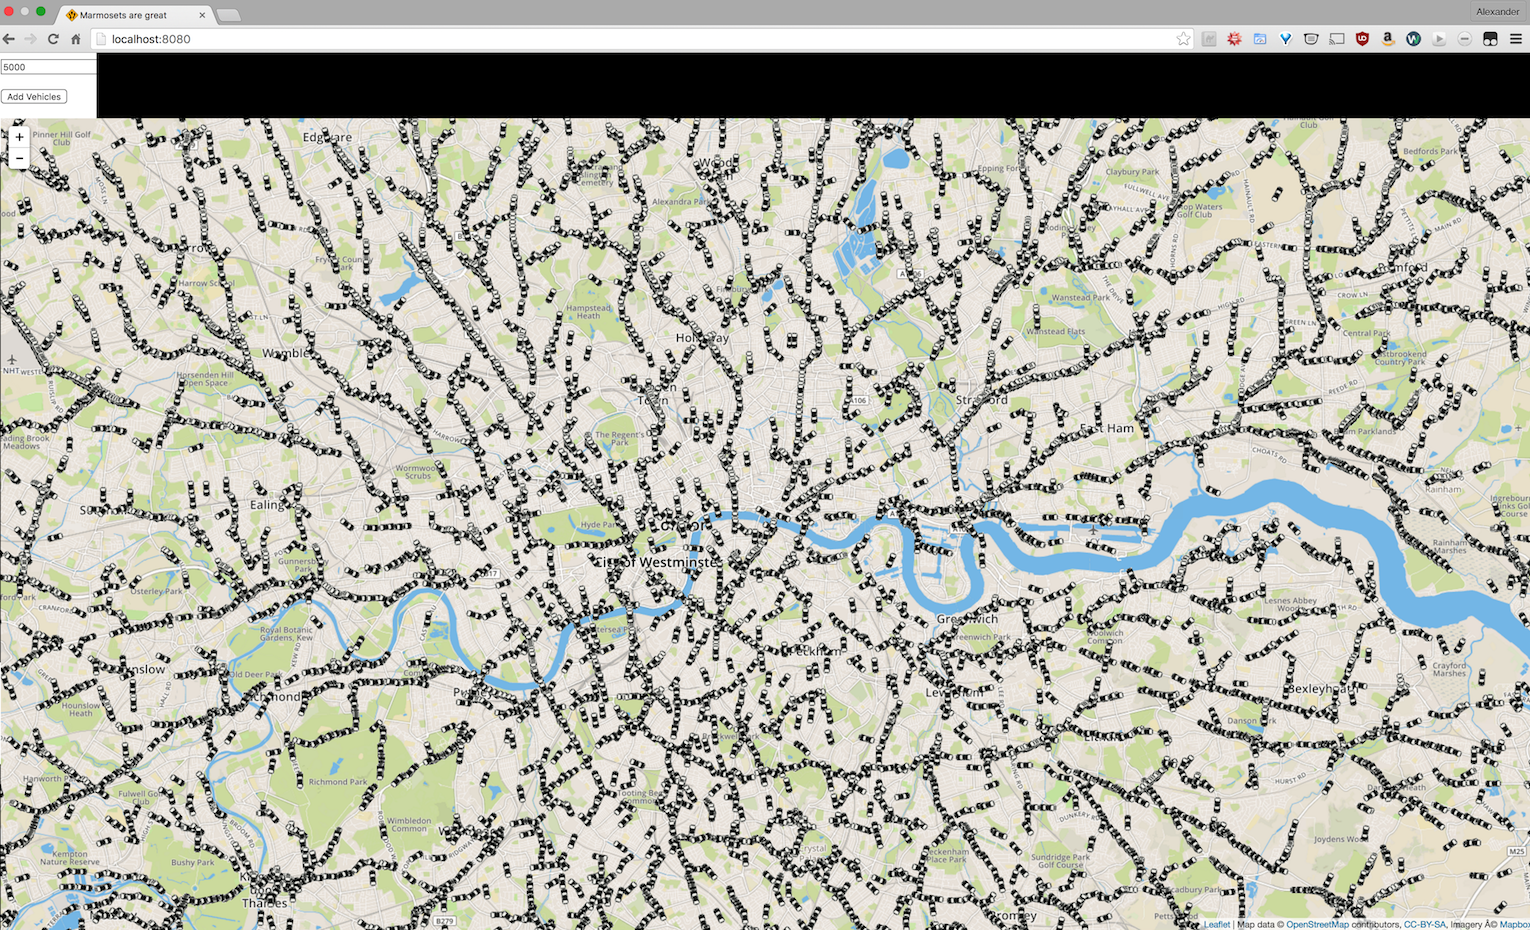
\includegraphics[height=9em]{glitches-chrome}
    \caption{Large black blocks showing over parts of the screen.}\label{fig:glitches-chrome}
\end{subfigure}
\caption{Graphical glitches caused by displaying more than 16,000 images.}
\end{figure}

\subsubsection{Marker Rendering}

I had initially used the Leaflet.AnimatedMarker library to make it appear as
though the vehicles are driving around the map in real time. However, this had a
huge performance cost, and as such had to be disabled.

Additionally, the vehicle image I used was reasonably large and in colour. I
created a much smaller vehicle image (from 15KB to 1KB.), which did improve
performance a little, but did not raise the 16,000 vehicle limitation.

One of the core issues with the existing implementation was the use of
\texttt{img} tags for displaying the vehicles. As each HTML tag is a full blown
element in the DOM, there is a reasonably high performance cost associated with
their use. There are two main alternatives for showing graphics in the browser -
SVG and the HTML5 Canvas API.

Unlike the img tag, the Canvas API is designed for drawing and other graphical
purposes. Instead of one tag per vehicle, A single \texttt{<canvas>} element
would be able to render every vehicle. I had been concerned that there would be
major challenges in extending the Leaflet Marker class to use an entirely
different way of showing markers, but thankfully Leaflet provided the location
to display the markers in pixels to marker subclasses. Using Canvas offered
drastically improved performance with seemingly no upper limit on how many
vehicles the front end could display with no glitches.

However, there were a few downsides to using Canvas. Firstly, the map correctly
re-rendered all the markers when zooming in and out, but not update the markers
when panning the map. Attempts at fixing this issue were unsuccessful.
Additionally, the img tags were able to support a popup when mousing over a
vehicle that showed its current speed and ID, which was useful for debugging.
This would have to be implemented by hand to be supported with Canvas - manually
detecting the current mouse position, checking which vehicle it was hovering
over and then drawing a custom popup on top of the view.
\begin{wrapfigure}{l}{0.35\textwidth}
    \begin{greybox}
        \centering
        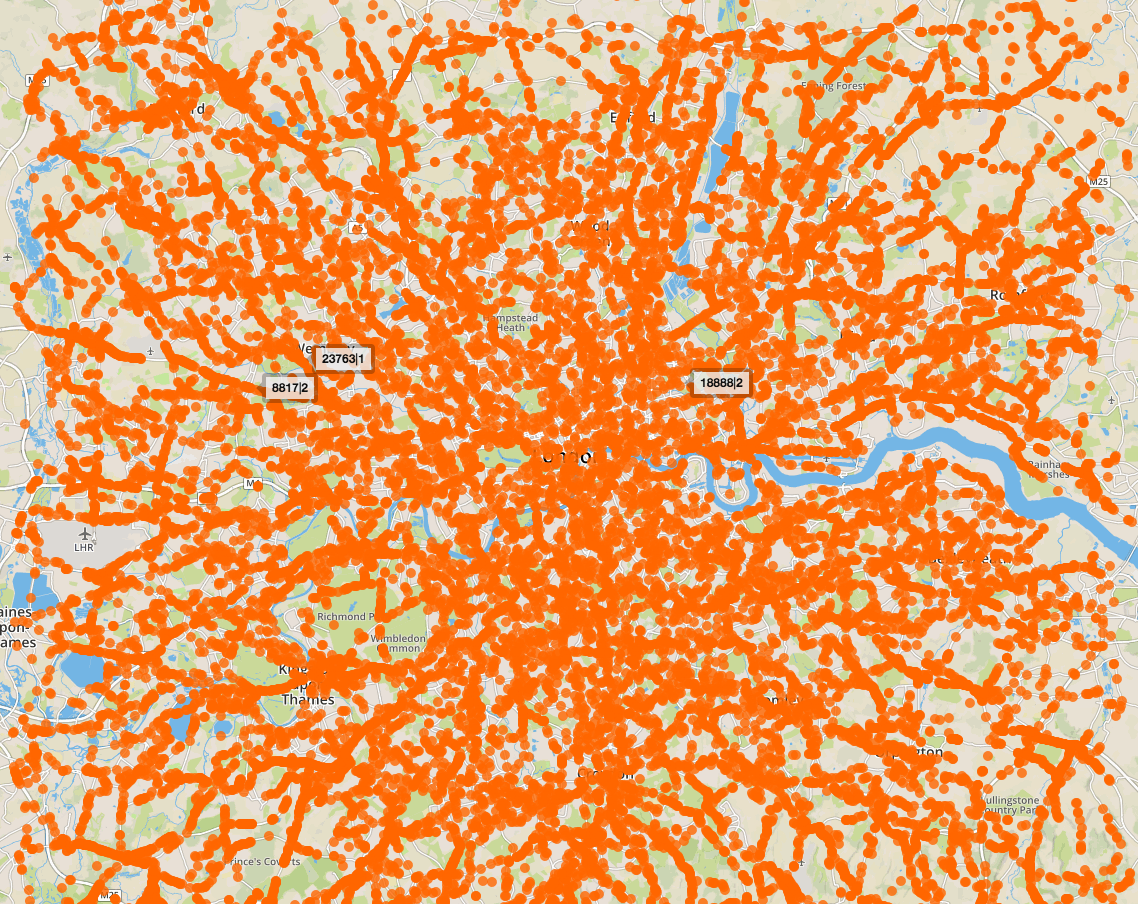
\includegraphics[width=\textwidth]{orange-markers}
        \caption{SVG Rendered orange markers showing 30,000 vehicles}\label{fig:orange-markers}
    \end{greybox}
    \vspace{-2em}
\end{wrapfigure}

Instead, I decided to experiment with SVG (Scalable Vector Graphics), an XML
based web API. One key advantage is that Leaflet has built in support for
drawing certain types of SVG elements. The static image marker could simply be
replaced with a \texttt{CircleMarker}, which used the same API as the Animated
and normal image markers but instead shows a circle with customisable radius and
colour.

SVG combined the performance of Canvas (rendering 64,000 vehicles whilst
remaining responsive) and the interactivity of img tags (panning around the map
worked flawlessly, and popups worked with no additional work). The only downside
was that a circle is shown instead of a vehicle icon, meaning it is not possible
to rotate the shape to indicate which direction the vehicles are travelling.
This is a minor price to pay for the performance improvements, so the decision
was made to use SVG for the front end moving forwards - the result can be seen
in Figure \ref{fig:orange-markers}.

\subsubsection{WebSocket Data Format}

The backend initially just sent down data in string format - for example,
\textit{10067|51.5306611887|0.1609468558|1} for vehicle with id 10067. This
format has a number of issuses. Firstly, there is limited precision for the
values, as they must be truncated to a certain number of decimal places.
Secondly, the format is text based, meaning there is a much larger overhead of
space compared to storing the values numerically. Finally, it takes additional
time to convert the data into a string only to parse it back into numerical
values on both the front end and back end.

The string data required for updating the locations of 1000 vehicles takes 33Kb.
Encoding this as raw binary data requires 4 bytes for the vehicle id and speed
each and 8 bytes for each of the latitude and longitude, requiring 24 bytes per
vehicle and hence 24Kb for the total transfer.  This is not only smaller, but
also comes with a performance and accuracy improvement as well.

Thankfully, the WebSocket protocol supports the sending of binary data, which
can then be efficiently processed by the front end using the DataView APIs. On
the back end, we create a single reusable BinaryBuffer object and pass it to the
Vehicles, which add their data into a specific offset. This is significantly
more efficient than the string based method, although the change is primarily
for improving network and front end performance.

\subsection{Back-end Performance}

\subsubsection{Removing timelock}

The most necessary change was removing the added delay for the timestep from the
Marmoset class. Instead of sending the data every second, the socket server
waits for a `next' message from the front end to start processing the next
timestep. It then sends the data and continues to wait for the command to
continue.

This drastically improved the speed of the system. For low numbers of vehicles,
each timestep takes little more than a few milliseconds on both the front and
back end. 1000 iterations with 1000 vehicles used to take at least 16 minutes -
after making this change it took just 50 seconds.

Additionally, this allowed much larger numbers of vehicles to be simulated and
visualised at the same time - the back end will only send data to the front end
once it has rendered the previous set of changes.

This also made it easier to add the ability to pause the simulation - by simply
ceasing to send the \texttt{next} message, the back end does no further work,
leaving the user able to explore the current state of the simulation in the
browser.

\subsubsection{Exploiting Parallelism}

Initial version of the system simply did all their work on a single thread.
There were a number of places were task level parallelism made it easy to add
more threads and cores to the system to improve performance.

\begin{lstlisting}[caption={The single-threaded \texttt{timestep} function},
    label=lst:timestep]
public void timestep()
{
    vehicles.stream().forEach(Vehicle::accelerationStep);
    vehicles.stream().forEach(Vehicle::slowStep);
    vehicles.stream().forEach(Vehicle::randomStep);
    vehicles.stream().forEach(Vehicle::moveStep);
    vehicles.stream().forEach(Vehicle::updateLocation);

    vehicles.stream().filter(v -> !v.isFinished()).collect(Collectors.toList());
}
\end{lstlisting}

In Listing \ref{lst:timestep} we can see the use of the Java 8 Stream API to run
the Nagel-Schreckenberg functions on each vehicle. However, one of the core
features of the API is built-in support for concurrency. By replacing the calls
to \texttt{stream()} with \texttt{parallelStream()}, Java will automatically
split the computation over multiple threads, whilst ensuring that all processes
have completed when the next line is executed. Minor changes were made to ensure
that the filter step for removing finished vehicles from the collection was
still thread-safe.

When adding new vehicles to the simulation, their initialisation uses
GraphHopper to find the route to their destination. This takes orders of
magnitude longer than the timesteps themselves, and as GraphHopper is
thread-safe for making routing requests is an easy way to further improve
performance.

EXPLAIN THIS BIT FURTHER MAYBE???

\subsection{Architecture Improvments}

One of the issues with the system at this point was the lack of support for
multiple vehicle types - although there is a Vehicle class that could have been
be subclassed, it was not easy to modify its behaviour without having to rewrite
large portions of the code.  As such, I decided a refactor of this part of the
system was required to improve the architecture of the system.

\subsubsection{Vehicle Refactoring}

\begin{figure}[h]
    \centering
    \includegraphics[scale=0.6,page=6,clip,trim=0 11cm 8cm 0]{architecture}
    \caption{The Vehicle and VehicleIterator class structure}\label{fig:veh-arch}
\end{figure}

Following the refactor, the Vehicle and VehicleIterator have been changed into
interfaces with the public methods originally implemented in the Vehicles class.
\texttt{BaseVehicle} and \texttt{BaseVehicleIterator} are abstract classes that
implement most of the boilderplate functionality. BaseVehicle holds the
implementation of the Nagel-Schreckenberg model, with routing behaviour defined
by the VehicleIterator. A subclass of BaseVehicle must implement only a single
method - \texttt{getVehicleIterator()}, which creates a VehicleIterator of the
correct type and with the right routing information.

For the standard routing algorithm, new \texttt{DijkstraVehicle} and
\texttt{DijkstraVehicleIterator} classes have been created. As a way of
verifying that multiple vehicle types are possible, I also created a
\texttt{RandomVehicle} and corresponding \texttt{RandomVehicleIterator} that
simply drive around at random with no overarching behaviour.

\subsection{Metric calculations}

The initial engine only allowed for viewing the results of an algorithm by
looking at the visualisation - it is also important to be able to perform
offline analysis of the data.

Brief calculations showed that storing the full movement of 64,000 vehicles
could take up to 10GB of storage, suggesting that it was better to calculate
metrics at each timestep and store those instead. There are three main types of
metric - vehicle, route and network metrics.

\subsubsection{Vehicle Metrics}

As their name suggests, vehicle metrics provide information about the state of
one or more vehicles. They can be calculated at any time, so can be recorded and
stored on each iteration. Vehicle metrics are the easiest way of getting a sense
of the overall behaviour of the system at any point in time.

With the goal of understanding the levels of congestion, I tracked two main
vehicle metrics: the number vehicles not moving at the maximum road speed, and
the number of vehicles that slowed down due to a vehicle in front of them.

A new inner \texttt{Metric} class was added to MarmosetHopper, with simple data
properties storing the average values for the two metrics mentioned above, as
well as the total number of vehicles and the average speed (in cells per second)
of the vehicles. The \texttt{toString} method has also been overridden to print
the data in CSV format, whilst a static method returns the header for the CSV
file to output.

\subsubsection{Route Metrics}

We can also better understand congestion by looking at how long a journey should
take compared to how long it did take. The GraphHopper \texttt{GHResponse} class
stores the length of time a route is expected to take. Although it does not
include a realistic model of vehicle behaviour (so does not truly represent the
correct time a journey would take, even on empty roads), the difference between
expected and actual time is another metric that can be used to compare different
vehicle behaviours.

Route metrics can only be recorded once the vehicle has reached its destination
rather than whilst it's travelling. As such, I added a \texttt{printMetrics}
function to BaseVehicle and provided implementations in DijkstraVehicle, which
prints the expected time from GraphHopper and the actual number of iterations
the vehicle took to reach its destination.

These metrics are output into a file that holds the id of the vehicle in
question - each vehicle has its own file, meaning there is no need for
centralised management of writing to disk.

\subsubsection{Network Metrics}

Network Metrics provide information about the roads themselves and how congested
or occupied they are. Instead of providing numerical data for every edge (which
provides very little information given how few cells/vehicles the average edge
has), a visual approach was used, simply retaining the full set of vehicle
positions and speed every 1000 iterations.

The code previously used to convert the Vehicle objects into strings was
repurposed and instead placed into an iteration file, meaning the data is human
readable and easy to parse. Adding a simple input box with basic parsing code
allows the data to be explored interactively after the simulation has finished,
as can be seen in Figure \ref{fig:offline-network}.

\begin{wrapfigure}{r}{0.4\textwidth}
    \vspace{-1em}
    \begin{greybox}
        \centering
        \includegraphics[width=\textwidth]{dijkstra-15k-wide}
        \caption{Post-simulation analysis of the 9,000th iteration of 15,000 vehicles}\label{fig:offline-network}
    \end{greybox}
    \vspace{-2em}
\end{wrapfigure}

\subsection{Event System}

Although the refactors mentioned above do allow for a large amount of
flexibility, using new vehicle classes (or adding new behaviour during existing
parts fo the process) required modifying the source of the engine directly.
Using a simple events system enables users of the engine to add code and
functionality during key points of the programs execution without directly
modifying the engine. Instead, users can call a \texttt{listenTo} method with a
callback function that is executed when the event is triggered.

Event triggers were added in key locations so that this features would be
useful. For example, an event is triggered at the start and end of each
timestep, at the beginning and end of initialisation and when a new vehicle is
added.

\subsection{Offline Simulation}

With the addition of metrics, it became clear that it would be useful to be able
to run a simulation in the background and analyse the data later. One use case
would be understanding how long it takes all vehicles to reach their
destinations - another is for analysing very high density networks where it may
not be desirable to view the data on screen.

A command line flag (\texttt{-{}-file}) was added representing the number of
vehicles to be simulated. The simulation creates a folder for the metrics
including the number of vehicles and a Unix timestamp, allowing it to be
uniquely identified.

However, the offline simulation appeared to be running slower than I had hoped
given it was not constrained by the browser rendering. The VisualVM Java
profiler was used to identify potential performance improvements whilst
simulating. Interestingly, far more time was spent in the
\texttt{updateLocation} step than I had expected - and given that the physical
location is only used for display and not internal routing, a flag was added to
disable the location updates for every timestep. Instead, the location is only
updated when required (e.g for outputting the locations every 1000 iterations).

\begin{figure}[h]
    \centering
    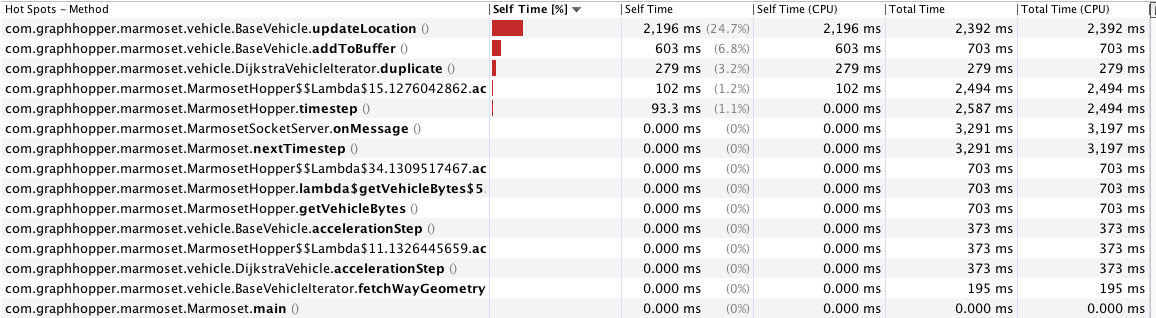
\includegraphics[width=0.9\textwidth,clip,trim=0 7cm 0 0]{visualvm-profile}
    \caption{VisualVM Profile of the most time consuming functions}\label{fig:visualvm}
\end{figure}

Removing the location updates had a drastic improvement to offline performance,
meaning simulations with large numbers of vehicles could be simulated to
completion in a reasonably short amount of time.

\section{Algorithm Design and Implementation}

As a way of exploring the capaiblity of the simulation engine, a multi-vehicle
routing algorithm was designed, implemented and tested.

\subsection{Algorithm Design}

I chose to design a V2I algorithm, as there would be a substantial amount of
additional code required to simulate realistic V2V communication. It is also
beneficial that V2I simulation can apply to both high and low density situations
as it is not limited by the distance to the nearest vehicle. Instead, access to
a central system that knew the location and planned destination of every vehicle
in a city was assumed. The algorithm would then provide routes for each vehicle
in the system.

The initial implementation of the Marmoset algorithm is described below. It is
important to note that this is not the final algorithm - the goal was to find a
potentially effective and then optimise and improve it using the simulation
engine. We will describe the behaviour of individual vehicles and the central
system separately.

\subsubsection{Vehicle Behaviour}

Individual vehicles make their current route and position available to
the central system at all times. The vehicles request routes from the system and
then follow them directly. A vehicle requests a new route after a random
interval (based on a predetermined parameter).

\subsubsection{Central System Behaviour}

The central system stores the number of vehicles that have been told to route
along each edge, called the Expected Map. It is initialised with zero values for
all edges on startup.

At a fixed interval, the system updates the expected map by multiplying every
edge by a damping factor that is less than 1. It then adds the edges in each
vehicle's current route to the expected map.

When a route is requested, the data from the expected map is used in conjunction
with a congestion function to modify the weight of edges based on their expected
density. This will return a route that avoids high-congestion roads, which will
be reflected in the expected map upon its next update.

A congestion function was chosen that was similar to the data found by
<RESEARCHERS/CONGESTION FUNCTION STUFF HERE>

\subsubsection{Design Justification}

The goal of the expected map is to help vehicles avoid roads that are likely to
have high levels of traffic. However, a naive approach to this would result in
oscillatory behaviour between optimal and suboptimal routes, as can be seen in
Figure \ref{fig:bjam-dijkstra} in Section \ref{sec:beejama}. As such, the expected map
is retained for further requests. Updating the expected map results first
multiplies each value by the damping factor. The goal of this is to stop the
system from having too much of a memory (and hence overpenalising roads that
will have many vehicles on them). This factor can be adjusted to define how much memory
the system will have of the vehicle's locations.

Furthermore, the system can handle the expectation that most routes will
change at some point whilst the vehicle is on the road. The random rerouting was
chosen partly for improved performance of the simulation and partly to ensure
that the busy areas will not be avoided entierly by all vehicles once the
expected map has shown that they will be busy. If every vehicle was rerouted
simultaneously, the vehicles would completely avoid the busy roads and hence
fail to use the network capacity available to them.

\subsection{Implementation}

The implement

\subsection{Testing}

%This chapter is intended to describe what you did: the goal is to explain
%the main activity or activities, of any type, which constituted your work
%during the project.  The content is highly topic-specific, but for many
%projects it will make sense to split the chapter into two sections: one
%will discuss the design of something (e.g., some hardware or software, or
%an algorithm, or experiment), including any rationale or decisions made,
%and the other will discuss how this design was realised via some form of
%implementation.

%This is, of course, far from ideal for {\em many} project topics.  Some
%situations which clearly require a different approach include:

%\begin{itemize}
%\item In a project where asymptotic analysis of some algorithm is the goal,
      %there is no real ``design and implementation'' in a traditional sense
      %even though the activity of analysis is clearly within the remit of
      %this chapter.
%\item In a project where analysis of some results is as major, or a more
      %major goal than the implementation that produced them, it might be
      %sensible to merge this chapter with the next one: the main activity
      %is such that discussion of the results cannot be viewed separately.
%\end{itemize}

%\noindent
%Note that it is common to include evidence of ``best practice'' project
%management (e.g., use of version control, choice of programming language
%and so on).  Rather than simply a rote list, make sure any such content
%is useful and/or informative in some way: for example, if there was a
%decision to be made then explain the trade-offs and implications
%involved.

% -----------------------------------------------------------------------------

\chapter{Critical Evaluation}
\label{chap:evaluation}

%{\bf A topic-specific chapter, of roughly $15$ pages}
%\vspace{1cm}

%\noindent
%This chapter is intended to evaluate what you did.  The content is highly
%topic-specific, but for many projects will have flavours of the following:

%\begin{enumerate}
%\item functional  testing, including analysis and explanation of failure
      %cases,
%\item behavioural testing, often including analysis of any results that
      %draw some form of conclusion wrt. the aims and objectives,
      %and
%\item evaluation of options and decisions within the project, and/or a
      %comparison with alternatives.
%\end{enumerate}

%\noindent
%This chapter often acts to differentiate project quality: even if the work
%completed is of a high technical quality, critical yet objective evaluation
%and comparison of the outcomes is crucial.  In essence, the reader wants to
%learn something, so the worst examples amount to simple statements of fact
%(e.g., ``graph X shows the result is Y''); the best examples are analytical
%and exploratory (e.g., ``graph X shows the result is Y, which means Z; this
%contradicts [1], which may be because I use a different assumption'').  As
%such, both positive {\em and} negative outcomes are valid {\em if} presented
%in a suitable manner.

% -----------------------------------------------------------------------------

\chapter{Conclusion}
\label{chap:conclusion}

%{\bf A compulsory chapter,     of roughly $5$ pages}
%\vspace{1cm}

%\noindent
%The concluding chapter of a dissertation is often underutilised because it
%is too often left too close to the deadline: it is important to allocation
%enough attention.  Ideally, the chapter will consist of three parts:

%\begin{enumerate}
%\item (Re)summarise the main contributions and achievements, in essence
      %summing up the content.
%\item Clearly state the current project status (e.g., ``X is working, Y
      %is not'') and evaluate what has been achieved with respect to the
      %initial aims and objectives (e.g., ``I completed aim X outlined
      %previously, the evidence for this is within Chapter Y'').  There
      %is no problem including aims which were not completed, but it is
      %important to evaluate and/or justify why this is the case.
%\item Outline any open problems or future plans.  Rather than treat this
      %only as an exercise in what you {\em could} have done given more
      %time, try to focus on any unexplored options or interesting outcomes
      %(e.g., ``my experiment for X gave counter-intuitive results, this
      %could be because Y and would form an interesting area for further
      %study'' or ``users found feature Z of my software difficult to use,
      %which is obvious in hindsight but not during at design stage; to
      %resolve this, I could clearly apply the technique of Smith [7]'').
%\end{enumerate}

% =============================================================================

% Finally, after the main matter, the back matter is specified.  This is
% typically populated with just the bibliography.  LaTeX deals with these
% in one of two ways, namely
%
% - inline, which roughly means the author specifies entries using the
%   \bibitem macro and typesets them manually, or
% - using BiBTeX, which means entries are contained in a separate file
%   (which is essentially a databased) then inported; this is the
%   approach used below, with the databased being dissertation.bib.
%
% Either way, the each entry has a key (or identifier) which can be used
% in the main matter to cite it, e.g., \cite{X}, \cite[Chapter 2}{Y}.

\backmatter

\bibliography{dissertation}

% -----------------------------------------------------------------------------

% The dissertation concludes with a set of (optional) appendicies; these are
% the same as chapters in a sense, but once signaled as being appendicies via
% the associated macro, LaTeX manages them appropriatly.

\appendix

\chapter{An Example Appendix}
\label{appx:example}

%Content which is not central to, but may enhance the dissertation can be
%included in one or more appendices; examples include, but are not limited
%to

%\begin{itemize}
%\item lengthy mathematical proofs, numerical or graphical results which
      %are summarised in the main body,
%\item sample or example calculations,
      %and
%\item results of user studies or questionnaires.
%\end{itemize}

%\noindent
%Note that in line with most research conferences, the marking panel is not
%obliged to read such appendices.

% =============================================================================

\end{document}
